%%%%%%%%%%%%%%%%%%%%%%%%%%%%%%%%%%%%%%%%%
% University Assignment Title Page
% LaTeX Template
% Version 1.0 (27/12/12)
%
% This template has been downloaded from:
% http://www.LaTeXTemplates.com
%
% Original author:
% WikiBooks (http://en.wikibooks.org/wiki/LaTeX/Title_Creation)
%
% License:
% CC BY-NC-SA 3.0 (http://creativecommons.org/licenses/by-nc-sa/3.0/)
%
%%%%%%%%%%%%%%%%%%%%%%%%%%%%%%%%%%%%%%%%%%
%\title{Title page with logo}
%----------------------------------------------------------------------------------------
%	PACKAGES AND OTHER DOCUMENT CONFIGURATIONS
%----------------------------------------------------------------------------------------

\documentclass[12pt]{article}

\usepackage{appendix}
%%% Работа с русским языком
\usepackage{cmap}					% поиск в PDF
\usepackage{mathtext} 				% русские буквы в формулах
\usepackage[T2A]{fontenc}			% кодировка
\usepackage[utf8]{inputenc}			% кодировка исходного текста
\usepackage[english,russian]{babel}	% локализация и переносы

\usepackage[nottoc]{tocbibind}
\usepackage{amsmath}
% \usepackage{indentfirst}
\usepackage{graphicx}
\usepackage{caption}
\usepackage{hyperref}
\hypersetup{
 colorlinks=true,
 linkcolor=black,
 citecolor=black,
 filecolor=black!30!green,      
 urlcolor=black!30!green,
}
\usepackage{subcaption}
\usepackage[colorinlistoftodos]{todonotes}
\usepackage{setspace}
\usepackage[natbibapa]{apacite} %this package helps set the right citation style
\usepackage{fullpage} %sets appropriate margins
\usepackage{geometry}
\geometry{
 a4paper,
 total={210mm,297mm},
 left=30mm,
 right=20mm,
 top=20mm,
 bottom=30mm,
 }

 
\usepackage{amsthm}
\usepackage[english]{babel}
\newtheorem{definition}{Definition}
\newtheorem{theorem}{Theorem}
\newtheorem{proposition}{Proposition}
\newtheorem{prediction}{Prediction}


\begin{document}
\bibpunct{(}{)}{;}{a}{,}{,}
 \onehalfspacing
\begin{titlepage}

\newcommand{\HRule}{\rule{\linewidth}{0.5mm}} % Defines a new command for the horizontal lines, change thickness here

\center % Center everything on the page
%\vspace*{-3.5cm}
%----------------------------------------------------------------------------------------
%	HEADING SECTIONS
%----------------------------------------------------------------------------------------

\textsc{правительство российской федерации}\\
\textsc{федеральное государственное автономное образовательное учреждение высшего профессионального образования}\\
\textsc{"Национальный исследовательский университет}\\
\textsc{"Высшая школа экономики"}\\[1cm] % Name of your university/college
%\textsc{\Large Major Heading}\\[0.5cm] % Major heading such as course name
%\textsc{\large Minor Heading}\\[0.5cm] % Minor heading such as course title

\textsc{негосударственное образовательное учреждение}\\
\textsc{высшего образования}\\
\textsc{"российская экономическая школа" (институт)}\\[2cm]

\textsc{\textmd{выпускная квалификационная работа}}\\[0.5cm]
%----------------------------------------------------------------------------------------
%	TITLE SECTION
%----------------------------------------------------------------------------------------
\begin{spacing}{1.5}
\HRule \\[0.4cm]
{ \huge \bfseries Общественные блага и отношение к этническому многообразию}\\[0.4cm] % Title of your document
\HRule \\[0.5cm]
\end{spacing}
%----------------------------------------------------------------------------------------
%	AUTHOR SECTION
%----------------------------------------------------------------------------------------

%\textsc{\textit{\large Бакалаврская программа}}\\[0.2cm]
\textsc{\textit{\large Программа Бакалавр экономики}}\\[0.2cm]
\textsc{\textit{\large Совместная программа по экономике НИУ ВШЭ и РЭШ}}\\[2cm]


\begin{minipage}{0.4\textwidth}
\begin{flushleft} \large
\emph{Автор:}\\
 \textsc{Иван Дедюхин} % Your name
 \vspace{2.5cm}
\end{flushleft}
\end{minipage}
~
\begin{minipage}{0.4\textwidth}
\begin{flushleft} \large
\emph{Научный руководитель:} \\
\textsc{Шломо Вебер} \\% Supervisor's Name
\vspace{1cm}
\emph{} \\
\textsc{} % Consultant's Name (if applicable)

\end{flushleft}
\end{minipage}\\[3cm]



%----------------------------------------------------------------------------------------
%	DATE SECTION
%----------------------------------------------------------------------------------------

{\large Москва, 2022 г.}%\\[2cm] % Date, change the \today to a set date if you want to be precise

%----------------------------------------------------------------------------------------
%	LOGO SECTION
%----------------------------------------------------------------------------------------

%\includegraphics{logo.png}\\[1cm] % Include a department/university logo - this will require the graphicx package

%----------------------------------------------------------------------------------------

\vfill % Fill the rest of the page with whitespace

\end{titlepage}

\begin{titlepage}

\newcommand{\HRule}{\rule{\linewidth}{0.5mm}} % Defines a new command for the horizontal lines, change thickness here

\center % Center everything on the page
%\vspace*{-3.5cm}
%----------------------------------------------------------------------------------------
%	HEADING SECTIONS
%----------------------------------------------------------------------------------------

\textsc{Higher School of Economics}\\
\textsc{}\\
\textsc{}\\
\textsc{}\\[1cm] % Name of your university/college
%\textsc{\Large Major Heading}\\[0.5cm] % Major heading such as course name
%\textsc{\large Minor Heading}\\[0.5cm] % Minor heading such as course title

\textsc{New Economic School}\\
\textsc{}\\
\textsc{}\\[2cm]

\textsc{\textmd{Bachelor’s Thesis
}}\\[0.5cm]
%----------------------------------------------------------------------------------------
%	TITLE SECTION
%----------------------------------------------------------------------------------------
\begin{spacing}{1.5}
\HRule \\[0.4cm]
{ \huge \bfseries Attitudes towards ethnic diversity and provision of public goods}\\[0.4cm] % Title of your document
\HRule \\[0.5cm]
\end{spacing}
%----------------------------------------------------------------------------------------
%	AUTHOR SECTION
%----------------------------------------------------------------------------------------

%\textsc{\textit{\large Бакалаврская программа}}\\[0.2cm]
\textsc{\textit{\large Bachelor of Arts in Economics}}\\[0.2cm]
\textsc{\textit{\large HSE-NES Joint Program}}\\[2cm]


\begin{minipage}{0.4\textwidth}
\begin{flushleft} \large
\emph{Author:}\\
 \textsc{Ivan Dedyukhin} % Your name
 \vspace{2.5cm}
\end{flushleft}
\end{minipage}
~
\begin{minipage}{0.4\textwidth}
\begin{flushleft} \large
\emph{Advisor:} \\
\textsc{Shlomo Weber} \\% Supervisor's Name
\vspace{1cm}
\emph{} \\
\textsc{} % Consultant's Name (if applicable)

\end{flushleft}
\end{minipage}\\[3cm]



%----------------------------------------------------------------------------------------
%	DATE SECTION
%----------------------------------------------------------------------------------------

{\large Moscow, 2022}%\\[2cm] % Date, change the \today to a set date if you want to be precise

%----------------------------------------------------------------------------------------
%	LOGO SECTION
%----------------------------------------------------------------------------------------

%\includegraphics{logo.png}\\[1cm] % Include a department/university logo - this will require the graphicx package

%----------------------------------------------------------------------------------------

\vfill % Fill the rest of the page with whitespace

\end{titlepage}

\begin{abstract}
Этническое разнообразие является важным фактором, определяющим количество общественного блага. Точный механизм не определен, и я вношу свой вклад, утверждая, что отношение к разнообразию имеет значение. Я разрабатываю модель и эмпирически показываю, что плохое отношение к этническому разнообразию приводит к уменьшению объема предоставляемых общественных благ. Эта статья предлагает новый механизм связи между этнической неоднородностью и обеспечением общественных благ.
\end{abstract}

\selectlanguage{english}
\begin{abstract}

Ethnic diversity is an essential determinant of public good provision. The exact mechanism is not defined and I contribute arguing that attitude towards diversity matters. I present the simple model and show empirically that a worse attitude towards ethnic diversity causes a decrease in the amount of provided public good. This paper proposes a new mechanism for the connection between ethnic heterogeneity and public good provision.

\end{abstract}


\newpage
\selectlanguage{english}

\tableofcontents

\selectlanguage{english}
\newpage

\section{Introduction}

Does ethnic diversity affect the provision of public goods, or is it only the attitude towards nationalities that matters? The answer to this question may have a beneficial influence on public policy towards ethnicities. This question is significant in Russia, mainly because it is multinational. In 2010 the index of ethnolinguistic diversity varied from 0.095 to 0.837 for Russian regions (\cite{Russia}). If the attitude towards heterogeneity matters, the state can start a policy of reconciliation to stop nationalism. If diversity matters, the government may not affect the regional division or the settlement of nationalities. Every answer to the stated research question is interesting for economists and politicians because of its effect on population welfare. 

I created a simple model where the economy consists of different agents that are belonged to different ethnicities. The agent's utility depends on the consumption of private and public goods, and the utility from consumption of public goods decreases in ethnic heterogeneity. I assume this mechanism because the consumption of public goods is associated with interaction with people that agents may not like. I show that a worse attitude towards ethnic diversity causes a decrease of provided public good amount.

To show the empirical effect, I used the US Census and Lincoln Institute of Land Policy data to construct alienation and fiscal variables for US cities. I have found that a worse attitude towards diversity causes a decrease in spending on parks and recreational facilities, education, and police.

The paper contributes to the literature on the connection between ethnic diversity and public good provision. It proposes a new mechanism of alienation. 

The paper is organized as follows. Section \ref{sec: literature} presents the overview of literature on the topic of relationship between ethnic polarization and public good provision. Section \ref{sec: model} describes the model. Section \ref{sec: empirics} presents the data description and empirical evidence. Section \ref{sec: discussion} elaborates on the possible drawbacks. Section \ref{sec: conclusion} concludes. 


\section{Literature review}
\label{sec: literature}

Ethnic diversity is an essential determinant of economic performance. For example, \cite{Africa} shows that ethnic diversity explains the difference in public policies between countries in Sub-Saharan Africa. These varieties explain lower economic growth in countries with higher ethnic fragmentation. 

Talking about public goods, the classical paper from \cite{AlesinaDivision} argues that the higher ethnic diversity is associated with the lower provision of some public goods. They presented a model in which different ethnic groups have different preferences for the public good to explain such dependence. They have found that spending on education, roads, sewers, and trash pickup is inversely related to fractionalization index, while police, health, and welfare had no effect. The endogeneity concern occurs here because the data was from US municipalities, and people may move between them. The paper from \cite{Kenya} deals with it because the ethnic patterns are stable and historically determined. They showed that ethnic fractionalization is associated with lower spending on primary schools. In addition, they presented a model based on the other mechanism of social sanctions. Higher ethnic fractionalization causes a failure of collective actions due to incapacity to implement sanctions. In addition, \cite{Indonesia} support all results of previous papers. The authors use the variation in ethnic fragmentation because of new jurisdictions and show that greater ethnic fractionalization causes increased deforestation. This is consistent with the paper on under provision of public goods. Moreover, the \cite{transfer} have found the same effect but presented a different mechanism. They argue that higher ethnic diversity increases the cost of producing public goods. It can be explained by the greater transaction costs and strengthened the problem of public action.

\cite{WhyUndermine} contributed to the mechanism of collective action. They ran several experiments and have found that the strategy selection mechanism is the main one. In similar conditions, agents from the same ethnic group play cooperative equilibrium, but agents from different groups do not. At the same time, they argue that the preferences mechanism is not the same one. However, \cite{Cooperation} have different results. They argue that evolutionary game theory predicts deviation from cooperative strategy, but social diversity helps deal with this problem. To prove that, the authors introduced an experiment with a public good game and showed that diversity promotes cooperation.

\cite{difference} argues that previous papers focused on fractionalization while the distance in social and economic characteristics also matters. They have found that economic inequality strengthens the effect shown in previous papers.

At this moment, it is crucial to elaborate on different polarization and fractionalization indexes. Firstly, \cite{Reynal-Querol} introduced polarization index instead of fractionalization. They argue that previous papers have shown a weak connection between fractionalization and conflict that explains a lower economic growth rate. The authors develop a new polarization index and show that it is better to explain the frequency of civil wars. Secondly, \cite{EstebanRay} introduced their theory of the measurement of polarization. They presented the polarization index and used it for analysis of ethnic diversity. \cite{EstebanRayConflict} distinguished between the occurrence of the conflict and its seriousness. They have shown that fractionalization and polarization tend to have opposite effects on both aspects, and the second one has a positive impact on the intensity of the conflict. These facts suggest that attitude toward ethnic diversity has a higher impact than its fragmentation. Other paper from \cite{alpha} presents different the family of polarization indices that I will use in the paper.

Talking about an attitude towards diversity, \cite{Foreign} explain determinants of attitudes towards foreigners and shows significant variation in the period from 1988 to 2008. \cite{Refuges} show that greater ethnic fractionalization and polarization are associated with lower support of refugees in Europe, which means a worse attitude to diversity. At the same time, this effect is not robust to different measures of ethnic diversity. 

Literature leaves me with the idea that attitude towards ethnic diversity affects public goods provision instead of actual fractionalization.

\section{Model}
\label{sec: model}

In this section, I will describe the baseline model. The economy consists of agents and ethnic groups. Each agent $i$ belongs to some ethnicity $I$, and this affiliation is exogenous. Different agents are endowed with varying levels of income. The set of nationalities $E$ is fixed. Firstly, I will follow \cite{BBV} model of private provision of public goods. Secondly, I will take a case of state provision of a public good, where the government is assumed to maximize social welfare.

\subsection{Setup}

The setup almost repeats the baseline theoretical model from \cite{BreakUp}. The economy population is $N$, and $p(I)$ is the ethnic group $I$ population. Hence
\[
    \sum_{I}p(I) = N
\]

I will define $\pi(I)$ as a share of ethnicity $I$  in total population of economy:
\[ \pi(I) = \frac{p(I)}{N} \]

Each agent's utility $u(x, g, H)$ depends on private consumption ($x$), public goods consumption ($g$), and ethnic heterogeneity ($H$). The utility function is twice continuously differentiable, strictly concave, and increasing in $x$ and $g$. For simplicity, the prices of private and public goods are set to 1. I assume that ethnic heterogeneity reduces the utility an agent derives from consuming the public good $g$. It happens because the consumption of public good requires communication with other people. An agent may not be satisfied because of interactions with other nationalities that he does not like. This is the main mechanism that I will discuss further. Also, I refuse the claim of the \cite{AlesinaDivision} that different ethnic groups might have different preferences over private and public consumption because \cite{WhyUndermine} refutes this mechanism. That is why the utility function is the same for all nationalities with given heterogeneity. 


\subsection{First best}

I will take the quasi-linear utility function with convex preferences. This function meets all the requirements described in the baseline. The utility of each agent $i$ from a group $I$ in country $C$ is 
\begin{equation}
\label{eq:utility}
U_i = x_i + \gamma((1 - H_i) g)^\beta    
\end{equation}
where $x_i$ is a private consumption of an agent $i$, $H_i$ is ethnic diversity that she faces, $g$ is an amount of public good. I will define $H(I)$ as a heterogeneity of each agent in group $I$. $\beta \in (0,1) $ implies convexity of preferences, and $\gamma$ implies the degree of preference for the public good in comparison with the private.

Let me suppose that the total income is W. The Samuelson condition (\cite{Samuelson}) gives us the first best allocation of resources.
\begin{equation}
    \label{eq:SC}
    \sum_{i = 1}^{N} MRS_i = 1
\end{equation}

\[ \sum_{I} p(I) \gamma(1-H(I))^\beta \beta g^{\beta - 1} = 1 \]

Hence, the Equation \ref{eq:FB} gives us the first best amount of public good

\begin{equation}
   g^{FB} = \left( \gamma\beta \sum_{I} p(I) (1-H(I))^{\beta} \right) ^\frac{1}{1 - \beta } 
   \label{eq:FB}
\end{equation}

\subsection{Private provision}

Suppose that public goods are specific to each country and are financed through private provision. 
The budget constraint for each agent is following
\[x_i(I) + g_i(I) \le  w_i(I) \]
where $w_i(I)$ is an income of agent from group $I$, $x_i(I)$ is private consumption of agent from group $I$,  and $g_i(I)$ is a contribution of an agent from group $I$. Utility function is increasing in private provision, so I claim that budget constraint is binding.

So, the utility function is
\[ U = w_i(I) - g_i(I) + \gamma( (1 - H(I) ) g)^\beta \] 
where $g$ is a total provision of public good.

The optimization problem for each agent is following:

\[ \max_{g_i > 0} w_i(I) - g_i(I) + \gamma( (1 - H(I)^\delta) (g_{-i} + g_i))^\beta  \]
where $g_{-i}$ is a total contribution of all other agents.
The solution of this problem leads to the following proposition.

\begin{proposition}
The amount of public good in the economy with its private provision decreases with the increase of ethnic heterogeneity for a group with the lowest diverseness.
\end{proposition}

\begin{proof}
The FOC is
\[ -1 + \beta\gamma (1 - H(I))^{\beta} ((g_i(I) + g_{-i} ))^{\beta-1} = 0 \]

\[ g_i(I) = \max \left\{\frac{1}{(\beta\gamma )^\frac{1}{\beta - 1} (1 - H(I))^\frac{\beta}{\beta-1} } - g_{-i} ; 0  \right\}   \]

We may notice that groups differ only in heterogeneity, and higher diversity cause a greater bliss amount. The wanted amount of a group $I$ with heterogeneity $H$ is 

\[ G(I) =  \frac{1}{(\beta\gamma )^\frac{1}{\beta - 1} (1 - H(I))^\frac{\beta}{\beta-1} } \]

The Nash equilibrium amount is the bliss amount for the group with the smallest heterogeneity. This group will contribute, and all others will contribute zero because their bliss amount is less, and their contribution will lead to an increase in the public good.

Hence 

\[g = \frac{1}{(\beta\gamma )^\frac{1}{\beta - 1} (1 - \min_{I} H(I))^\frac{\beta}{\beta-1} } \]

\begin{equation}
    g^{PP} = (\beta\gamma  ( 1 - \min_{I} H(I)))^\frac{\beta}{1 -\beta}
    \label{eq:privat}
\end{equation}

where $g^{PP}$ is an equilibrium amount for the economy with private provision of public good. It is decreasing in $\min_{I} H(I)$, thus higher ethnic heterogeneity for the group that faces the lowest heterogeneity decreases the total provision of public good. 
\end{proof}

\subsubsection{Alienation effect}

For theoretical purposes, the measure of ethnic diversity will be the weighted attitudes distance between that resident and all other residents of the economy. This corresponds to the expected distance between an agent from a region $I$ and a randomly drawn agent from the economy. The greater distance means a worse attitude and greater heterogeneity.

\[ H(I) = \sum_{J} \frac{p(J) \alpha(I, J)}{N} = \sum_{J} \pi(J) \alpha(I,J) \]
where $\alpha(I, J)$ is an attitude of group $I$ towards the group $J$ (distance between groups). Important to say that $\alpha(I, J) \ne \alpha(J, I)$. Let me suppose that the identification $\alpha(I,I) = 0$ for all $I$ for all $C$. I will call $\alpha(I, J)$ alienation if $I \ne J$. I chose that form because the attitude ($\alpha$) and probability to meet ($\frac{p(J)}{p(C)}$) matters the satisfaction of public good.

Now suppose two groups: ethnic minority(1) and ethnic majority(2). Majority and minority means that $\pi(1) < \pi(2)$ Alienation is $\alpha(1,2) = \alpha_1$; $\alpha(2,1) = \alpha_2$, and identification is $\alpha(1,1) = \alpha(2,2) = 0$. Hence, we may say that
\[ H(1) = \sum_{J} \frac{p(J) \alpha(1, J)}{N} = \pi(2) * \alpha_1 \]
\[ H(2) = \sum_{J} \frac{p(J) \alpha(2, J)}{N} = \pi(1) * \alpha_2 \]
Also for simplicity let me define $\pi_1 = \pi(1)$ and $\pi_2 = \pi(2)$

\begin{proposition}
    Increase in alienation of any group causes a decrease or immutability in public good provision.
\end{proposition}

\begin{proof}
From, the previous results and equation \ref{eq:privat} we can notice that

\[ g^{PP} = \min \left\{ (\beta\gamma  ( 1 - \min_{I} H(I)))^\frac{\beta}{1 -\beta}; W( \text{argmin}_{I} H(I)) \right\} \]

Hence we had two cases:
\begin{enumerate}
    \item $H(1) > H(2)$:
    \[ g^{PP} = \min \left\{ (\beta\gamma  ( 1 - H(2)))^\frac{\beta}{1 -\beta}; W(2) \right\} \]
    The heterogeneity does not influence the income, so let me see the the internal solution.
    \[ g^{PP} (\beta\gamma  ( 1 - H(2)))^\frac{\beta}{1 -\beta} \]
    \[ g^{PP} (\beta\gamma  ( 1 - \pi_1 * \alpha_2))^\frac{\beta}{1 -\beta} \]
    Greater alienation of minor group causes decreases the amount of public good, while alienation of major group does not.
    
    \item $H(2) \ge H(1)$:
    \[ g^{PP} = \min \left\{ (\beta\gamma  ( 1 - H(1)))^\frac{\beta}{1 -\beta}; W(1) \right\} \]
    The heterogeneity does not influence the income, so let me see the the internal solution.
    \[ g^{PP} (\beta\gamma  ( 1 - H(1)))^\frac{\beta}{1 -\beta} \]
    \[ g^{PP} (\beta\gamma  ( 1 - \pi_2 * \alpha_1))^\frac{\beta}{1 -\beta} \]
    Greater alienation of major group causes decreases the amount of public good, while alienation of minor group does not.
    
    \item Increase in $\alpha$ cause a change of group:
    
    In this case, the minimal heterogeneity will not become lower because higher alienation does not cause a decrease in heterogeneity. Hence, greater alienation will cause a decrease or immutability of public good provision.
    
\end{enumerate}

\end{proof}

This result is logical because it increases the heterogeneity of one group without decreasing the heterogeneity for others. So, this is a consequence of proposition 1. 

\subsection{State provision}

Let me assume that government is benevolent and maximizes social welfare. The financing of public goods goes through tax as a percent of income. The optimization problem for the government is

\[ \max_{t\in[0,1], g\ge 0} \sum_{I} p(I) ( (1-t)w_i(I) + \gamma( (1 - H(I)) g)^\beta)  \]
\[ g \le t\sum_{I} p(I) w_i(I)  \]

\begin{proposition}
Higher heterogeneity for at least one ethnic group leads to lower provision of public good.
\end{proposition}

\begin{proof}

\[ g = t\sum_{I} p(I) w_i(I)  \]
because the social welfare is increasing in public good provision. 
Also, let me set $W = \sum_{I} p(I) w_i(I) $ as a total income. Hence $g = tW$, and
\[ \max_{t\in[0,1]} (1-t) W + \sum_{I} p(I) \gamma( (1 - H(I)) tW)^\beta)  \]
The FOC is 
\[ -W + \sum_{I} p(I) \gamma ((1 - H(I))^\beta W^\beta \beta t^{\beta - 1} = 0 \]

\[t = \min \left\{ \left( \gamma W^{\beta - 1} \beta\sum_{I} p(I) (1 - H(I))^\beta \right)^\frac{1}{1 - \beta}; 1 \right\} \]

\begin{equation}
    g^{SP} = \min \left\{ \left( \gamma  \beta\sum_{I} p(I) (1 - H(I))^\beta \right)^\frac{1}{1 - \beta}; W \right\}
    \label{eq:public}
\end{equation}

The provision of public good is decreasing in $H(I,C)$
\end{proof}

In addition, the Equation \ref{eq:public} gives us the amount of public good in the situation of state provision.

\subsubsection{Alienation effect}

Let me take the same heterogeneity form as in the case of private provision.

\begin{proposition}
    Increase in alienation of any group causes a decrease in public good provision.
\end{proposition}

\begin{proof}
    From equation \ref{eq:public} I have 
    \[ g^{SP} = \min \left\{ \left( \gamma  \beta\sum_{I} p(I) (1 - H(I))^\beta \right)^\frac{1}{1 - \beta}; W \right\} \]
    The heterogeneity does not affect income, so let me elaborate on the inner solution.
    \[ g^{SP} = \left( \gamma  \beta \left( p(1) (1 - \pi_2\alpha_1)^\beta + p(2) (1 - \pi_1\alpha_2)^\beta  \right) \right)^\frac{1}{1 - \beta} \]
    Increase in any $\alpha$ cause a decrease of the amount of public good.
\end{proof}

The theoretical analysis of different cases of economy with a private or state provision of public good gives the prediction that I will check empirically.

\begin{prediction}
    Alienation have negative effect on the amount of public good provided.
\end{prediction}

\subsection{Comparison}

In this section I want to compare the amount of public good that I got in equations \ref{eq:FB}, \ref{eq:privat}. and \ref{eq:public}. Hence, I want to compare first best, private provision, and state provision, respectively. Let me for simplicity assume that income is as great that we can neglect it. In this case amounts are following:

\[  g^{FB} = \left( \gamma\beta \sum_{I} p(I) (1-H(I))^{\beta} \right) ^\frac{1}{1 - \beta }  \]

\[ g^{PP} =  (\beta\gamma  ( 1 - \min_{I} H(I)))^\frac{\beta}{1 -\beta} \]

\[  g^{SP} = \left( \gamma  \beta\sum_{I} p(I) (1 - H(I))^\beta \right)^\frac{1}{1 - \beta}\]

We can notice that state provision of public goods leads to the first best amount of public goods, but it does not mean that it leads to the first-best allocation of contributions to the public good and its efficiency.

\begin{proposition}
If $N < (\beta\gamma)^{\beta-1}$ than the public good amount in the case of state provision is lower than in the case of private provision
\end{proposition}

\begin{proof}
    Let me compare in the case of equal heterogeneity $H$ that all groups faces

    \[ g^{PP} =  (\beta\gamma  ( 1 - H)^\frac{\beta}{1 -\beta}\;\;\; \bigvee \;\;\; g^{SP} = \left( \gamma  \beta\sum_{I} p(I) (1 - H)^\beta \right)^\frac{1}{1 - \beta} \]

    \[  (\beta\gamma)^{\beta-1}  (1 - H)^\beta \;\;\; \bigvee \;\;\;  N (1 - H)^\beta \]

    \[  (\beta\gamma)^{\beta-1} \;\;\; \bigvee \;\;\;  N \]

    Hence, if $N < (\beta\gamma)^{\beta-1}$, then the amount of public good with state provision is greater than in a situation with private provision. The case of different heterogeneity may be interpreted as an increase of some $H(I)$ compared to the considered case. So, the amount of state provision decreases while the amount of private provision stays the same.
\end{proof}

\begin{figure}[h!]
    \centering
    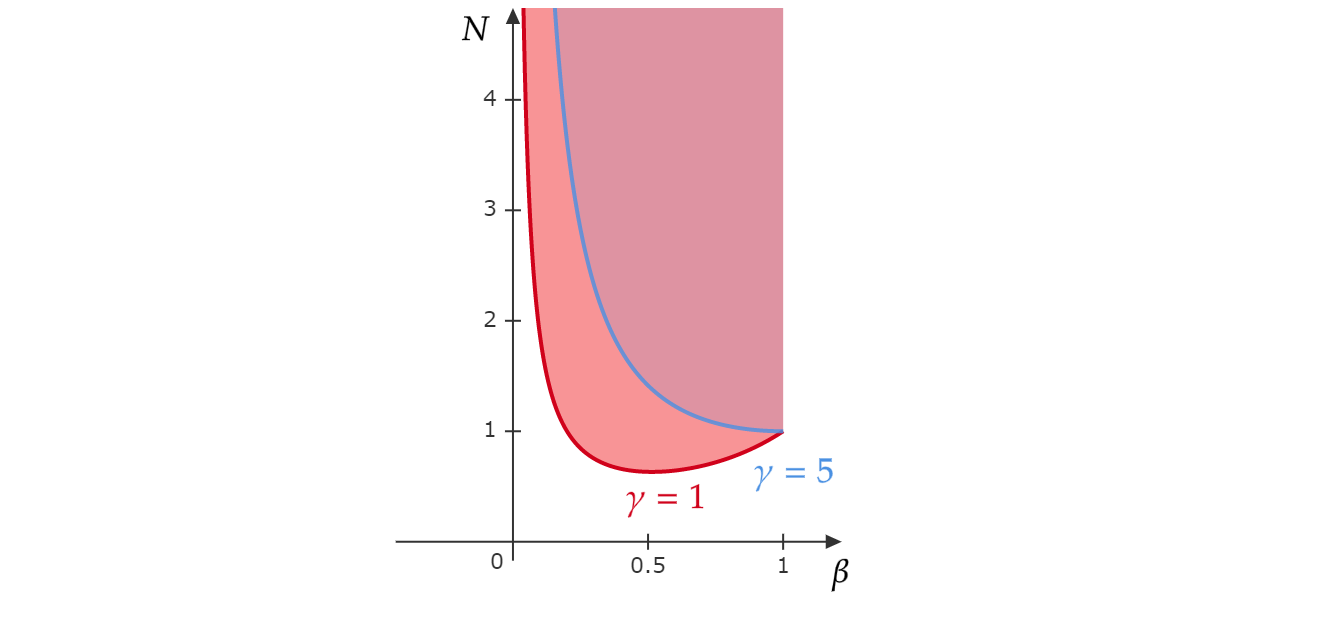
\includegraphics[scale = 0.3]{Thesis/Figures/picture model.png}
    \caption{Areas when state provision public good amount is greater in case of equal heterogeneity.}
    \label{fig:param}
\end{figure}

Figure \ref{fig:param} shows the area when state provision public good amount is greater for different parameters in case of equal heterogeneity. It turns out that we can say that a greater population means that, more likely, the state provision amount will be greater than the private provision amount. At the same time, if agents stronger prefer public good (increase in $\gamma$), then the state provision amount will be greater more likely.


\section{Empirical evidence}
\label{sec: empirics}

I test my predictions with a panel dataset of
public goods spending, ethnic diversity and attitudes towards it in 97  U.S. cities for the period 2006 - 2017.

\subsection{Data and sources}

I use the ethnic fractionalization (FRAC) and Reynal-Querol polarization (RQ) indices to measure ethnic heterogeneity. FRAC measures the probability that two randomly drawn people from a city belong to different ethnic groups. I will consider the population distribution by race, so I construct FRAC as follows:

\begin{equation}
    FRAC = \sum_{i} \pi_i (1 - \pi_i) = 1 - \sum_{i}\pi_i^2
\end{equation}
where $pi_i$ is a share of race $i$ in cities population and
\[ i \in \{\text{White, Black, Asian and Pacific Islander, American Indian, Other} \} \]

RQ is trying to intuitively capture how far the group distribution is from a bipolar distribution. Hence, I construct RQ as follows:
\begin{equation}
    RQ=1-\sum_{i=1}^{N}\left[\frac{0.5-\pi_{i}}{0.5}\right]^{2} \pi_{i}
\end{equation}

These indices are highly correlated in collected dataset. This fact is shown in the Figure \ref{fig:rq-frac}, which repeats the one from \cite{Reynal-Querol}.

\begin{figure}[h!]
    \centering
    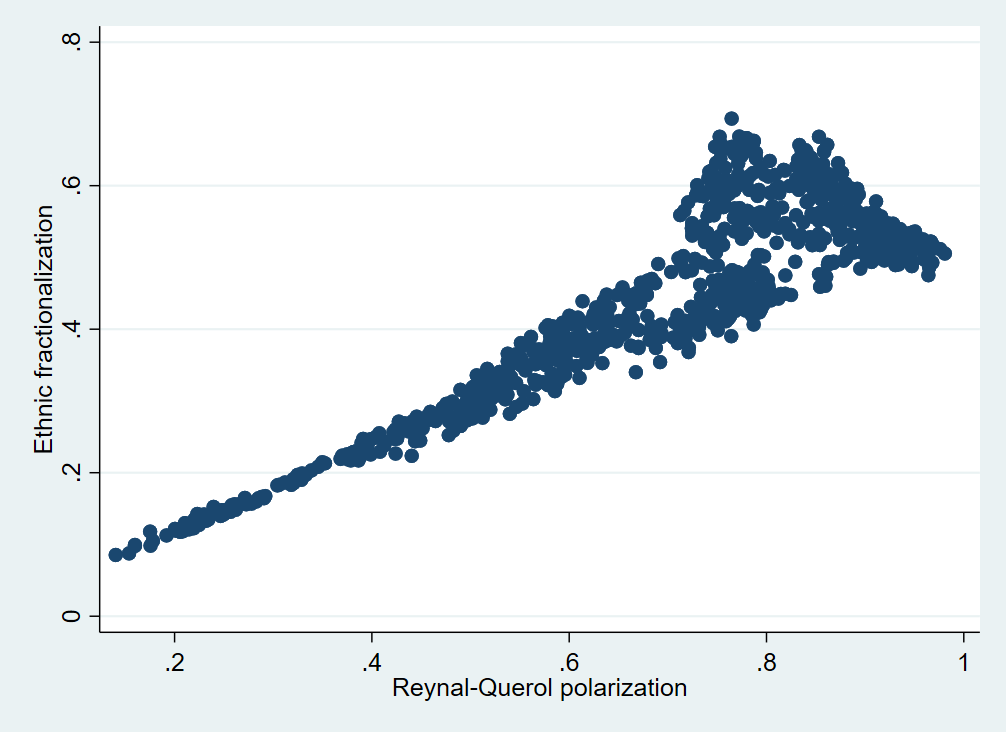
\includegraphics[scale = 0.3]{Thesis/Figures/frac-rq.png}
    \caption{Corellation between Reqnal-Querol and fractionalization indices}
    \label{fig:rq-frac}
\end{figure}

I follow the racial classification used by the U. S. Census. The source of the data is \hyperlink{https://usa.ipums.org/usa/}{IPUMS USA}  project that collects, preserves, and harmonizes U.S. census microdata. I had data on randomly drawn people from U.S. counties, so my identification strategy has the first assumption that balancing property holds for races at the city level. This database was also used to construct some controls as mean household income and inequality calculated by dividing average income by median one.

Note that there is no "Hispanic" option in racial classifications in the Census. However, there is a correlation (0.54) between "Hispanic" and "Other" in the above classification. Many Hispanics respond "Other" because they do not feel accurately represented in the multiple racial choice provided by the Census.

The attitude towards diversity index (ALIENATION) is created by myself. I calculate the share of co-racial marriages in a city's total number of marriages. I assume that the greater fraction causes less tolerance to diversity for the city's population. The possible caveat is that this INDEX is dependent on fractionalization because higher ethnic heterogeneity increases the probability of co-racial marriage.
Figure \ref{fig:frac-index} shows significant variation in attitudes towards diversity for the same ethnic fractionalization. Therefore, I argue that marriage represents alienation rather than ethnic heterogeneity.

\begin{figure}[h!]
    \centering
    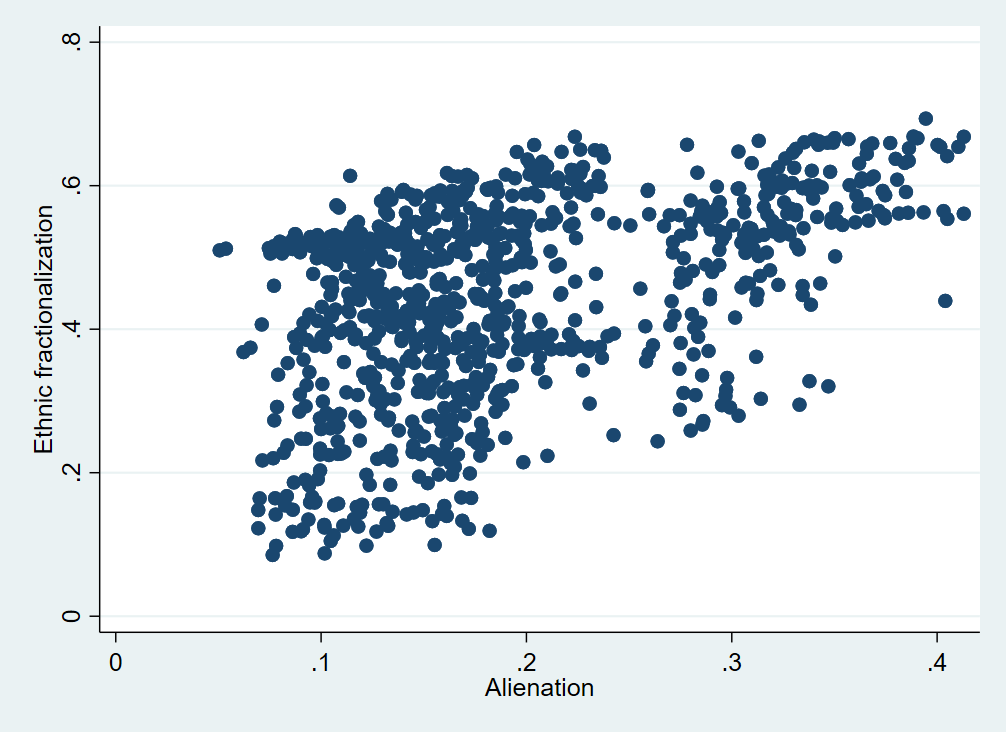
\includegraphics[scale =0.3]{Thesis/Figures/frac-index.png}
    \caption{Scatter plot for attitude index and ethnic fractionalization}
    \label{fig:frac-index}
\end{figure}

I have also calculated ethnic fractionalization among married people because some specific factors may influence decision about marriage and ethnic fractionalization. I have found no difference of this fractionalization with general diversity as probability of two random people be from different ethnic groups. The Figure \ref{fig:frac-frac} shows a strict correlation (0.98) between two indices.

\begin{figure}[h!]
    \centering
    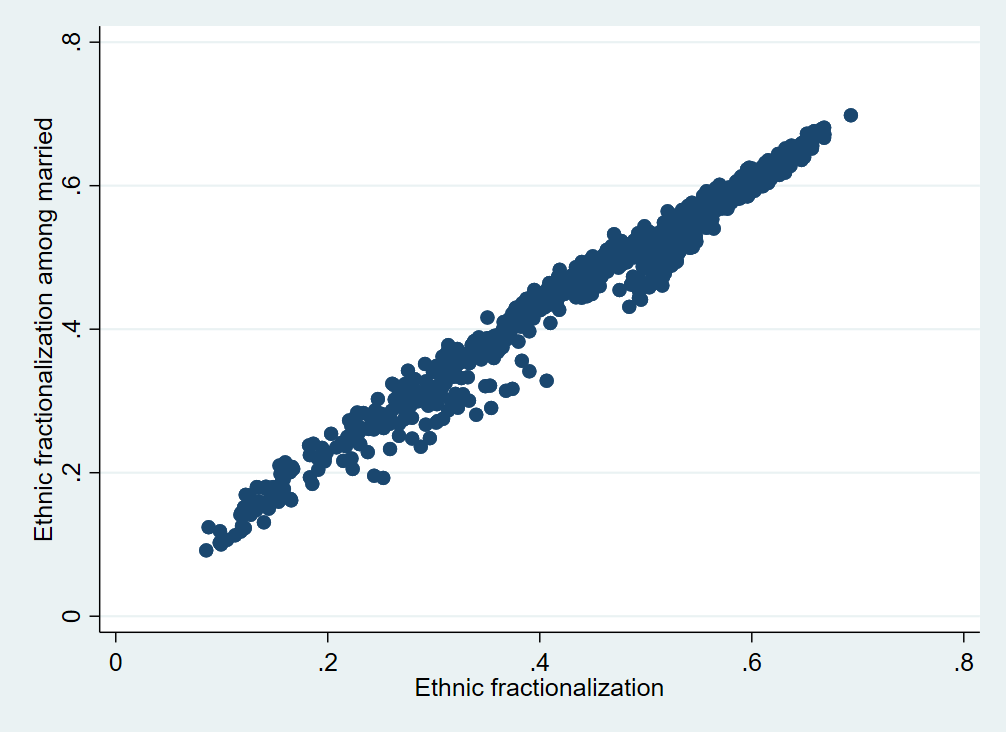
\includegraphics[scale = 0.3]{Thesis/Figures/frac-frac.png}
    \caption{Scatter plot for general fractionalization and fractionalization among married}
    \label{fig:frac-frac}
\end{figure}

Fiscal variables are taken from The Fiscally Standardized Cities (FiSC) database from Lincoln Institute of Land Policy. This database makes it possible to compare cities' finances because of different levels of government finance public goods and spending. The data are available for 212 US cities for the 1977–2017 period on the Lincoln Institute of Land Policy's \hyperlink{https://www.lincolninst.edu/research-data/data-toolkits/fiscally-standardized-cities}{website}. I have taken public spending variable by goals, city population, and taxes collected. All fiscal variables are calculated per capita in 2017 USD.

Fiscal and IPUMS datasets were merged by the year and city name. Descriptive statistics is presented in the Table \ref{tab:desc}. We can notice the significant variation in all variables of interest: ethnic fractionalization or polarization and attitude towards diversity. Figure \ref{fig:map} shows the geographical variation of cities in the sample. It seems to be sufficient to claim that merging two datasets reveals random cities from the US. The descriptive statistics also support this. 

\begin{figure}[h!]
    \centering
    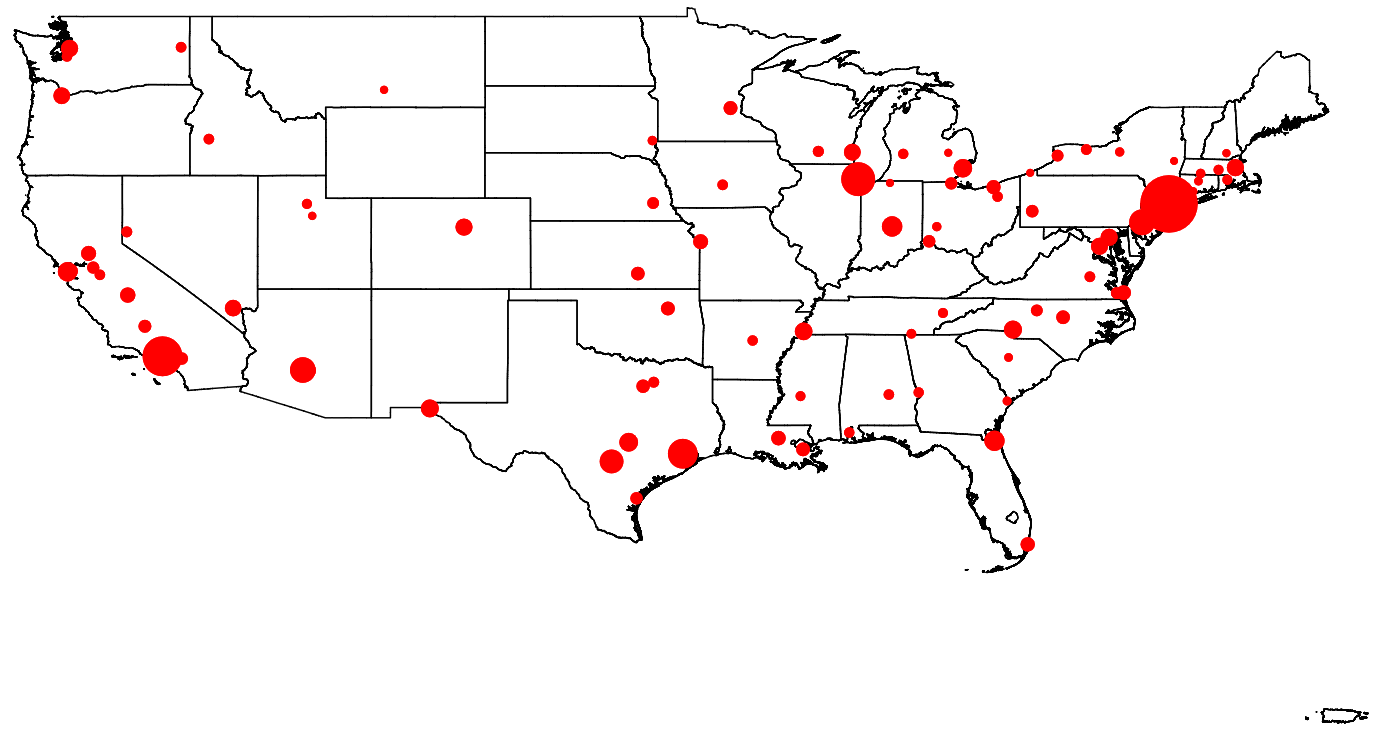
\includegraphics[scale = 0.35]{Thesis/Maps/city_population.png}
    \caption{The map of the U.S. cities used in dataset}
    \label{fig:map}
\end{figure}

\begin{table}[h!]
    \centering
    {
\def\sym#1{\ifmmode^{#1}\else\(^{#1}\)\fi}
\begin{tabular}{l*{1}{cccc}}
\hline\hline
                    &\multicolumn{4}{c}{(1)}                            \\
                    &\multicolumn{4}{c}{}                               \\
                    &        Mean&          S.D.&         Min&         Max\\
\hline
City Population     &    557022.8&     1060585&       80215&     8475976\\
Log of city population&    12.68124&    .8683314&    11.29247&    15.95275\\
Taxes collected     &    2198.987&    1221.208&      732.71&    11223.87\\
General expenditures&    5952.036&    2291.052&     2033.46&    21446.74\\
Secondary education expenditures&    2007.007&    644.0921&      544.84&     4811.56\\
Libraries expenditures&    51.92246&    34.49064&           0&      585.74\\
Public welfare expenditures&    268.4206&    604.8267&           0&     5725.41\\
Hospital expenditures&    282.1485&     582.429&           0&     4432.26\\
Health expenditures &    217.3635&    228.5996&           0&     2198.96\\
Highways expenditures&    232.4785&    133.0477&        6.21&     1067.75\\
Public safety expenditures&    773.3932&    265.9719&      268.43&     2312.49\\
Sewerage expenditures&    245.4629&    160.8913&           0&     1070.79\\
Administration expenditures&    308.1253&    168.1048&       56.07&     1698.06\\
Parks and recreation expenditures&    178.9966&    136.8253&        1.03&     1410.71\\
Ethnic fractionalization&    .4420603&    .1377596&    .0853811&    .6934802\\
Ethnic fractionalization among married&    .4580479&    .1321692&    .0917879&    .6981086\\
Reynal-Querol polarization&    .6988702&    .1972032&     .140374&    .9807938\\
Alienation          &     .189907&    .0825309&    .0536585&    .4158192\\
Mean HH income      &    634356.8&    404314.1&    88548.67&     2851736\\
Inequality          &    11.32726&    7.060934&    1.225278&     47.1012\\
\hline
Observations        &         900&            &            &            \\
\hline\hline
\end{tabular}
}

    \caption{Descriptive statistic for US cities 2006 - 2017}
    \label{tab:desc}
\end{table}

\subsection{Empirical estimations}

The Basic specification is 

\begin{equation}
\label{eq: basic}
    Fiscal_{it} = \alpha + \beta_1 \times FRAC_{it} + \beta_2 \times INDEX_{it} + \beta_3 \times INDEX_{it} \times FRAC_{it} + \gamma X_i + f_t + f_i + \epsilon_{it}
\end{equation}
where $X_i$ are covariates.

Previous papers have shown that $\beta_1$ is negative. My theoretical predictions and hypothesis expects $\beta_2$ and $\beta_3$ to be negative. The coefficient $\beta_2$ is responsible for the effect of attitude itself, and $\beta_3$ is responsible for complementarity. The subsection \ref{subsec: alienation} explores the effect of attitude towards heterogeneity while subsection \ref{subsec: complement} shows complementarity of fractionalization and index.

\begin{table}[h!]
    \centering
    \scriptsize
    {
\def\sym#1{\ifmmode^{#1}\else\(^{#1}\)\fi}
\begin{tabular}{l*{6}{c}}
\hline\hline
                    &\multicolumn{1}{c}{(1)}&\multicolumn{1}{c}{(2)}&\multicolumn{1}{c}{(3)}&\multicolumn{1}{c}{(4)}&\multicolumn{1}{c}{(5)}&\multicolumn{1}{c}{(6)}\\
                    &\multicolumn{1}{c}{Secondary education}&\multicolumn{1}{c}{Social services}&\multicolumn{1}{c}{Libraries}&\multicolumn{1}{c}{Parks}&\multicolumn{1}{c}{Police}&\multicolumn{1}{c}{Welfare}\\
\hline
Ethnic fractionalization&     -0.0317         &    -0.00455         &     -0.0104         &    0.000741         &     -0.0141         &    -0.00247         \\
                    &    (0.0555)         &    (0.0427)         &   (0.00721)         &    (0.0286)         &    (0.0303)         &    (0.0200)         \\
[1em]
Alienation          &      0.0938         &    -0.00811         &     -0.0171         &     -0.0431         &     -0.0332         &    -0.00416         \\
                    &     (0.116)         &    (0.0892)         &    (0.0151)         &    (0.0597)         &    (0.0632)         &    (0.0419)         \\
[1em]
Index x Frac        &      0.0141         &      0.0376         &      0.0450         &      0.0110         &      0.0557         &      0.0283         \\
                    &     (0.239)         &     (0.184)         &    (0.0311)         &     (0.123)         &     (0.131)         &    (0.0864)         \\
[1em]
Mean HH income      &    3.92e-08\sym{***}&   -2.94e-08\sym{***}&    1.08e-09         &   -9.99e-09         &   -1.04e-08         &    3.33e-09         \\
                    &  (1.14e-08)         &  (8.81e-09)         &  (1.49e-09)         &  (5.89e-09)         &  (6.24e-09)         &  (4.13e-09)         \\
[1em]
Inequality          &    -0.00188\sym{**} &     0.00148\sym{**} &   0.0000261         &    0.000489         &    0.000510         &   -0.000354         \\
                    &  (0.000728)         &  (0.000561)         & (0.0000946)         &  (0.000375)         &  (0.000397)         &  (0.000263)         \\
[1em]
Log of city population&       0.145\sym{***}&      0.0387         &    -0.00155         &     -0.0393\sym{*}  &     -0.0140         &      0.0196         \\
                    &    (0.0326)         &    (0.0251)         &   (0.00423)         &    (0.0168)         &    (0.0178)         &    (0.0118)         \\
[1em]
Constant            &      -1.476\sym{***}&      -0.383         &      0.0326         &       0.536\sym{*}  &       0.314         &      -0.211         \\
                    &     (0.415)         &     (0.319)         &    (0.0539)         &     (0.214)         &     (0.226)         &     (0.150)         \\
\hline
Observations        &         900         &         900         &         900         &         900         &         900         &         900         \\
\hline\hline
\multicolumn{7}{l}{\footnotesize Standard errors in parentheses}\\
\multicolumn{7}{l}{\footnotesize \sym{*} \(p<0.05\), \sym{**} \(p<0.01\), \sym{***} \(p<0.001\)}\\
\end{tabular}
}
    \caption{OLS general regression}
    \label{tab:basic}
\end{table}

\subsubsection{Alienation effect}
\label{subsec: alienation}

Firstly, I want to identify effect of the attitudes towards diversity. Simple OLS model is not applicable here because of multicollinearity of attitude index and ethnic fractionalization. The proof of multicollinearity is presented in Table \ref{tab:frac - index}

\begin{table}[h!]
    \centering
    \scriptsize
    {
\def\sym#1{\ifmmode^{#1}\else\(^{#1}\)\fi}
\begin{tabular}{l*{6}{c}}
\hline\hline
                    &\multicolumn{1}{c}{(1)}&\multicolumn{1}{c}{(2)}&\multicolumn{1}{c}{(3)}&\multicolumn{1}{c}{(4)}&\multicolumn{1}{c}{(5)}&\multicolumn{1}{c}{(6)}\\
                    &\multicolumn{1}{c}{Alienation}&\multicolumn{1}{c}{Alienation}&\multicolumn{1}{c}{Alienation}&\multicolumn{1}{c}{Alienation}&\multicolumn{1}{c}{Alienation}&\multicolumn{1}{c}{Alienation}\\
\hline
Ethnic fractionalization&       0.272\sym{***}&       0.136\sym{***}&       0.124\sym{***}&       0.290\sym{***}&       0.137\sym{***}&       0.117\sym{***}\\
                    &    (0.0490)         &    (0.0343)         &    (0.0319)         &    (0.0483)         &    (0.0329)         &    (0.0320)         \\
                    &                     &                     &   (0.00412)         &                     &                     &   (0.00511)         \\
[1em]
Mean HH income      &                     &                     &                     &    6.36e-08         &    1.90e-08         &   -9.28e-09         \\
                    &                     &                     &                     &  (3.61e-08)         &  (1.16e-08)         &  (1.12e-08)         \\
[1em]
Inequality          &                     &                     &                     &    -0.00545\sym{*}  &   -0.000182         &    0.000454         \\
                    &                     &                     &                     &   (0.00253)         &  (0.000683)         &  (0.000770)         \\
[1em]
Log of city population&                     &                     &                     &     0.00181         &      0.0333         &     -0.0270         \\
                    &                     &                     &                     &   (0.00913)         &    (0.0290)         &    (0.0336)         \\
[1em]
Constant            &      0.0698\sym{***}&       0.130\sym{***}&       0.128\sym{***}&      0.0600         &      -0.303         &       0.473         \\
                    &    (0.0191)         &    (0.0152)         &    (0.0146)         &     (0.117)         &     (0.370)         &     (0.427)         \\
\hline
Observations        &         900         &         900         &         900         &         900         &         900         &         900         \\
\hline\hline
\multicolumn{7}{l}{\footnotesize Standard errors in parentheses}\\
\multicolumn{7}{l}{\footnotesize \sym{*} \(p<0.05\), \sym{**} \(p<0.01\), \sym{***} \(p<0.001\)}\\
\end{tabular}
}

    \caption{Relationship between attitude and heterogeneity.}
    \label{tab:frac - index}
\end{table}

I will use propensity-score-matching and estimate the dose-response function with alienation as a treatment. \cite{prop} define propensity function as the conditional density of the actual treatment given the observed covariates. Hence, weak unconfoundedness holds, and \cite{prop} shows that the GPS (generalized propensity score) can be used to eliminate any biases associated with differences in the covariates.

Firstly, using \cite{package} STATA package that helps estimate dose-response function, I calculated propensity function with covariates fractionalization, polarization, mean income, inequality, taxes, and city population.
\[ r(t, x)=f_{T \mid X}(t \mid x) \]
Secondly, I estimate the conditional expectation of
the outcome as a function of two scalar variables, the treatment level T and the GPS R:
\[ \beta(t, r)=E(Y \mid T=t, R=r) \]
The form is following:
\[ Fiscal_i = \alpha + \beta_1 \times INDEX_i + \beta_2 \times GPS_i + \beta_3 \times INDEX_i \times GPS_i \]
In the third step, I finally estimate the dose–response function,
\[ \mu(t)=E[\beta\{t, r(t, X)\}] \]
This method helps me get fractionalization and polarization fixed and focus only on alienation.

Results are presented in Table \ref{tab:prop_score}. We can notice the expected and significant results only for secondary education, parks, and police fiscal dependent variable. Social services and public welfare are increased with greater alienation, and it can be caused by the inability of collective action to help a neighbor.

I have shown that the alienation and attitude towards diversity are essential determinants of public goods provision.

\begin{table}[h!]
    \centering
    \scriptsize
    {
\def\sym#1{\ifmmode^{#1}\else\(^{#1}\)\fi}
\begin{tabular}{l*{6}{c}}
\hline\hline
                    &\multicolumn{1}{c}{(1)}&\multicolumn{1}{c}{(2)}&\multicolumn{1}{c}{(3)}&\multicolumn{1}{c}{(4)}&\multicolumn{1}{c}{(5)}&\multicolumn{1}{c}{(6)}\\
                    &\multicolumn{1}{c}{Parks}&\multicolumn{1}{c}{Libraries}&\multicolumn{1}{c}{ Education}&\multicolumn{1}{c}{Police}&\multicolumn{1}{c}{Welfare}&\multicolumn{1}{c}{Social services}\\
\hline
Alienation          &     -0.0367\sym{*}  &     0.00555         &      -0.219\sym{**} &     -0.0710\sym{**} &       0.215\sym{***}&       0.175\sym{*}  \\
                    &    (0.0184)         &   (0.00448)         &    (0.0823)         &    (0.0262)         &    (0.0315)         &    (0.0749)         \\
[1em]
GPS&     0.00105         &     0.00114\sym{***}&    -0.00225         &    -0.00573\sym{**} &    0.000328         &    -0.00915         \\
                    &   (0.00128)         &  (0.000311)         &   (0.00571)         &   (0.00182)         &   (0.00219)         &   (0.00520)         \\
[1em]
Alienation \times GPS      &    -0.00401         &    -0.00479\sym{***}&      0.0244         &      0.0157\sym{*}  &    -0.00175         &      0.0208         \\
                    &   (0.00559)         &   (0.00136)         &    (0.0249)         &   (0.00793)         &   (0.00954)         &    (0.0227)         \\
[1em]
Constant            &      0.0369\sym{***}&     0.00685\sym{***}&       0.389\sym{***}&       0.159\sym{***}&    -0.00626         &      0.0980\sym{***}\\
                    &   (0.00500)         &   (0.00121)         &    (0.0223)         &   (0.00710)         &   (0.00854)         &    (0.0203)         \\
\hline
Observations        &         900         &         900         &         900         &         900         &         900         &         900         \\
\hline\hline
\multicolumn{7}{l}{\footnotesize Standard errors in parentheses}\\
\multicolumn{7}{l}{\footnotesize \sym{*} \(p<0.05\), \sym{**} \(p<0.01\), \sym{***} \(p<0.001\)}\\
\end{tabular}
}

    \caption{Propensity score matching results}
    \label{tab:prop_score}
\end{table}

These results are slightly consistent with results of general OLS modifications of specification \ref{eq: basic} in Tables \ref{tab: parks} - \ref{tab: social service} in Appendix. The only robust result in both strategies is parks and recreational spending. Park is a place where people meet each other. The greater alienation towards people in the park will decrease the utility from consuming this public good.

\subsubsection{Complementarity effect}
\label{subsec: complement}

Basic OLS regression from specification \ref{eq: basic} is presented in Table \ref{tab:basic}. So, we can not see a significant effect because of the high probability of multicollinearity. At the same time, we can see some significant complementary effect evidence in Table \ref{tab: parks} in specifications (3) and (6) or Table \ref{tab: libraries} in the specification (3), but this result is not robust. Hence, I decided to use the same propensity-score matching because I need the effect for given fractionalization and other covariates. The results are presented in Table \ref{tab:interaction}. I have found that the effect of alienation and actual diversity on public good provision is complementary to that that requires social interactions like parks and libraries. This result is consistent with the suggested mechanism.

\begin{table}[h!]
    \centering
    \scriptsize
    {
\def\sym#1{\ifmmode^{#1}\else\(^{#1}\)\fi}
\begin{tabular}{l*{6}{c}}
\hline\hline
                    &\multicolumn{1}{c}{(1)}&\multicolumn{1}{c}{(2)}&\multicolumn{1}{c}{(3)}&\multicolumn{1}{c}{(4)}&\multicolumn{1}{c}{(5)}&\multicolumn{1}{c}{(6)}\\
                    &\multicolumn{1}{c}{Parks}&\multicolumn{1}{c}{Libraries}&\multicolumn{1}{c}{Secondary education}&\multicolumn{1}{c}{Police}&\multicolumn{1}{c}{Welfare}&\multicolumn{1}{c}{Social services}\\
\hline
Index x Frac        &      -0.121\sym{**} &     -0.0192         &      -0.844\sym{***}&      -0.335\sym{***}&      0.0401         &       0.499\sym{**} \\
                    &    (0.0468)         &    (0.0114)         &     (0.210)         &    (0.0672)         &    (0.0815)         &     (0.192)         \\
[1em]
Alienation          &      0.0516\sym{*}  &      0.0128\sym{*}  &       0.159         &       0.138\sym{***}&       0.176\sym{***}&     -0.0889         \\
                    &    (0.0234)         &   (0.00572)         &     (0.105)         &    (0.0336)         &    (0.0407)         &    (0.0960)         \\
[1em]
GPS&    0.000546         &    0.000275\sym{*}  &    -0.00534\sym{*}  &    -0.00290\sym{***}&   -0.000115         &    -0.00240         \\
                    &  (0.000505)         &  (0.000123)         &   (0.00227)         &  (0.000726)         &  (0.000879)         &   (0.00207)         \\
[1em]
interaction         &    -0.00853\sym{*}  &    -0.00285\sym{**} &      0.0675\sym{***}&      0.0132\sym{*}  &     0.00405         &     0.00281         \\
                    &   (0.00368)         &  (0.000899)         &    (0.0165)         &   (0.00529)         &   (0.00641)         &    (0.0151)         \\
[1em]
Constant            &      0.0331\sym{***}&     0.00792\sym{***}&       0.401\sym{***}&       0.152\sym{***}&    -0.00381         &      0.0986\sym{***}\\
                    &   (0.00414)         &   (0.00101)         &    (0.0186)         &   (0.00595)         &   (0.00721)         &    (0.0170)         \\
\hline
Observations        &         900         &         900         &         900         &         900         &         900         &         900         \\
\hline\hline
\multicolumn{7}{l}{\footnotesize Standard errors in parentheses}\\
\multicolumn{7}{l}{\footnotesize \sym{*} \(p<0.05\), \sym{**} \(p<0.01\), \sym{***} \(p<0.001\)}\\
\end{tabular}
}

    \caption{Estimating the complementarity effect}
    \label{tab:interaction}
\end{table}


\section{Discussion}
\label{sec: discussion}

This section will discuss some possible drawbacks of the bachelor thesis.

There are some extensions for the model. The first and the most obvious one is that transaction costs may occur. It is hard to cooperate in societies with greater heterogeneity. That is why the producing costs of the public good may depend on heterogeneity in society. The main conclusion will not change because higher costs will decrease the provided amount so that ethnic heterogeneity will have another channel of influence.

The result is robust only for parks because the effect is significant in OLS and propensity-score estimations. It is not robust for libraries and secondary education because of differences between general OLS regression controlling for fractionalization and propensity score dose-response estimation. A more complex robustness check requires more covariates, including unemployment, criminal level, population density, etc.  

The other possible concern is about different levels of public spending. County's government may maximize the welfare of the county where the city is just a part of it. That is why citizens' preferences may not be taken into account by the county government. Hence, I may have a bias in my estimations. A possible solution for that is to control for a part of the costs funded by the county.

The other possible concern is the economic significance of the found results. It is hard to elaborate on the magnitude of the effect because it is hard to interpret my alienation index. The results are probably not economically significant, and the ethnic agenda is not important to policymakers. That is why future research is needed.


\section{Conclusion}
\label{sec: conclusion}

This is the first view on the impact of attitudes towards ethnic diversity on the public good provision. Further research may include better calculation of alienation and construction of attitudes of every group to every group. Surveys about attitudes towards heterogeneity may construct better alienation. The construction of attitudes of every group to every group may impact the results of the research because cities with general attitudes towards diversity seem not to suffer from ethnic tensions between two groups, while others are tolerant. That may influence all ways of life, including public good production.
\newpage

\bibliographystyle{apacite}
\bibliography{ref}


%\setcounter{secnumdepth}{0}
\newpage

\appendix

\section{Regressions results from basic specification}

\begin{table}[h!]
    \centering
    \scriptsize
  {
\def\sym#1{\ifmmode^{#1}\else\(^{#1}\)\fi}
\begin{tabular}{l*{6}{c}}
\hline\hline
                    &\multicolumn{1}{c}{(1)}&\multicolumn{1}{c}{(2)}&\multicolumn{1}{c}{(3)}&\multicolumn{1}{c}{(4)}&\multicolumn{1}{c}{(5)}&\multicolumn{1}{c}{(6)}\\
                    &\multicolumn{1}{c}{Parks}&\multicolumn{1}{c}{Parks}&\multicolumn{1}{c}{Parks}&\multicolumn{1}{c}{Parks}&\multicolumn{1}{c}{Parks}&\multicolumn{1}{c}{Parks}\\
\hline
Ethnic fractionalization&     -0.0416\sym{**} &     -0.0354\sym{**} &                     &     -0.0445\sym{***}&     -0.0317\sym{*}  &                     \\
                    &    (0.0125)         &    (0.0133)         &                     &    (0.0128)         &    (0.0143)         &                     \\
[1em]
Alienation          &                     &     -0.0227         &      0.0630         &                     &     -0.0453\sym{*}  &      0.0352         \\
                    &                     &    (0.0175)         &    (0.0408)         &                     &    (0.0175)         &    (0.0414)         \\
[1em]
Index x Frac        &                     &                     &      -0.176\sym{**} &                     &                     &      -0.164\sym{*}  \\
                    &                     &                     &    (0.0615)         &                     &                     &    (0.0629)         \\
[1em]
Mean HH income      &                     &                     &                     &    5.82e-09         &    8.45e-09         &    9.02e-09         \\
                    &                     &                     &                     &  (7.06e-09)         &  (6.61e-09)         &  (6.91e-09)         \\
[1em]
Inequality          &                     &                     &                     &   -0.000830\sym{*}  &    -0.00106\sym{*}  &    -0.00111\sym{*}  \\
                    &                     &                     &                     &  (0.000403)         &  (0.000421)         &  (0.000427)         \\
[1em]
Log of city population&                     &                     &                     &     0.00443\sym{*}  &     0.00446\sym{*}  &     0.00449\sym{*}  \\
                    &                     &                     &                     &   (0.00215)         &   (0.00204)         &   (0.00199)         \\
[1em]
Taxes collected     &                     &                     &                     &-0.000000691         &-0.000000574         &-0.000000573         \\
                    &                     &                     &                     &(0.000000904)         &(0.000000805)         &(0.000000768)         \\
[1em]
Constant            &      0.0496\sym{***}&      0.0512\sym{***}&      0.0350\sym{***}&     0.00204         &     0.00520         &    -0.00964         \\
                    &   (0.00612)         &   (0.00637)         &   (0.00435)         &    (0.0289)         &    (0.0278)         &    (0.0283)         \\
\hline
Observations        &         900         &         900         &         900         &         900         &         900         &         900         \\
\hline\hline
\multicolumn{7}{l}{\footnotesize Standard errors in parentheses}\\
\multicolumn{7}{l}{\footnotesize \sym{*} \(p<0.05\), \sym{**} \(p<0.01\), \sym{***} \(p<0.001\)}\\
\end{tabular}
}

    \caption{Results on share spent on parks and recreational facilities}
    \label{tab: parks}
\end{table}

\begin{table}[h!]
    \centering
    \scriptsize
  {
\def\sym#1{\ifmmode^{#1}\else\(^{#1}\)\fi}
\begin{tabular}{l*{6}{c}}
\hline\hline
                    &\multicolumn{1}{c}{(1)}&\multicolumn{1}{c}{(2)}&\multicolumn{1}{c}{(3)}&\multicolumn{1}{c}{(4)}&\multicolumn{1}{c}{(5)}&\multicolumn{1}{c}{(6)}\\
                    &\multicolumn{1}{c}{Libraries}&\multicolumn{1}{c}{Libraries}&\multicolumn{1}{c}{Libraries}&\multicolumn{1}{c}{Libraries}&\multicolumn{1}{c}{Libraries}&\multicolumn{1}{c}{Libraries}\\
\hline
Ethnic fractionalization&    -0.00957\sym{**} &    -0.00900\sym{**} &                     &    -0.00890\sym{**} &    -0.00808         &                     \\
                    &   (0.00286)         &   (0.00339)         &                     &   (0.00337)         &   (0.00412)         &                     \\
[1em]
Alienation          &                     &    -0.00207         &      0.0178         &                     &    -0.00290         &      0.0136         \\
                    &                     &   (0.00539)         &    (0.0121)         &                     &   (0.00575)         &    (0.0140)         \\
[1em]
Index x Frac        &                     &                     &     -0.0419\sym{*}  &                     &                     &     -0.0354         \\
                    &                     &                     &    (0.0167)         &                     &                     &    (0.0199)         \\
[1em]
Mean HH income      &                     &                     &                     &    2.60e-10         &    4.28e-10         &    7.70e-10         \\
                    &                     &                     &                     &  (2.01e-09)         &  (2.11e-09)         &  (2.05e-09)         \\
[1em]
Inequality          &                     &                     &                     &  -0.0000530         &  -0.0000680         &  -0.0000948         \\
                    &                     &                     &                     &  (0.000127)         &  (0.000138)         &  (0.000131)         \\
[1em]
Log of city population&                     &                     &                     &   -0.000210         &   -0.000208         &   -0.000249         \\
                    &                     &                     &                     &  (0.000505)         &  (0.000504)         &  (0.000502)         \\
[1em]
Taxes collected     &                     &                     &                     &   -2.08e-08         &   -1.33e-08         &   -4.11e-08         \\
                    &                     &                     &                     &(0.000000283)         &(0.000000284)         &(0.000000278)         \\
[1em]
Constant            &      0.0133\sym{***}&      0.0134\sym{***}&     0.00941\sym{***}&      0.0161\sym{*}  &      0.0163\sym{*}  &      0.0135         \\
                    &   (0.00141)         &   (0.00146)         &   (0.00129)         &   (0.00642)         &   (0.00649)         &   (0.00715)         \\
\hline
Observations        &         900         &         900         &         900         &         900         &         900         &         900         \\
\hline\hline
\multicolumn{7}{l}{\footnotesize Standard errors in parentheses}\\
\multicolumn{7}{l}{\footnotesize \sym{*} \(p<0.05\), \sym{**} \(p<0.01\), \sym{***} \(p<0.001\)}\\
\end{tabular}
}

    \caption{Results on share spent on libraries}
    \label{tab: libraries}
\end{table}

\newpage

\begin{table}[h!]
    \centering
    \scriptsize
  {
\def\sym#1{\ifmmode^{#1}\else\(^{#1}\)\fi}
\begin{tabular}{l*{6}{c}}
\hline\hline
                    &\multicolumn{1}{c}{(1)}&\multicolumn{1}{c}{(2)}&\multicolumn{1}{c}{(3)}&\multicolumn{1}{c}{(4)}&\multicolumn{1}{c}{(5)}&\multicolumn{1}{c}{(6)}\\
                    &\multicolumn{1}{c}{Education}&\multicolumn{1}{c}{Education}&\multicolumn{1}{c}{Education}&\multicolumn{1}{c}{Education}&\multicolumn{1}{c}{Education}&\multicolumn{1}{c}{Education}\\
\hline
Ethnic fractionalization&     -0.0750         &     -0.0349         &                     &      0.0623         &      0.0809         &                     \\
                    &    (0.0691)         &    (0.0704)         &                     &    (0.0681)         &    (0.0622)         &                     \\
[1em]
Alienation          &                     &      -0.147         &      0.0557         &                     &     -0.0656         &      -0.189         \\
                    &                     &     (0.149)         &     (0.270)         &                     &     (0.123)         &     (0.228)         \\
[1em]
Index x Frac        &                     &                     &      -0.360         &                     &                     &       0.288         \\
                    &                     &                     &     (0.400)         &                     &                     &     (0.411)         \\
[1em]
Mean HH income      &                     &                     &                     &    6.23e-08         &    6.61e-08         &    6.06e-08         \\
                    &                     &                     &                     &  (5.34e-08)         &  (5.38e-08)         &  (5.34e-08)         \\
[1em]
Inequality          &                     &                     &                     &    -0.00271         &    -0.00305         &    -0.00262         \\
                    &                     &                     &                     &   (0.00335)         &   (0.00333)         &   (0.00337)         \\
[1em]
Log of city population&                     &                     &                     &     -0.0271\sym{*}  &     -0.0270\sym{*}  &     -0.0261\sym{*}  \\
                    &                     &                     &                     &    (0.0108)         &    (0.0108)         &    (0.0108)         \\
[1em]
Taxes collected     &                     &                     &                     &  -0.0000316\sym{**} &  -0.0000314\sym{***}&  -0.0000308\sym{**} \\
                    &                     &                     &                     &(0.00000933)         &(0.00000920)         &(0.00000909)         \\
[1em]
Constant            &       0.389\sym{***}&       0.399\sym{***}&       0.377\sym{***}&       0.732\sym{***}&       0.737\sym{***}&       0.756\sym{***}\\
                    &    (0.0282)         &    (0.0310)         &    (0.0273)         &     (0.129)         &     (0.131)         &     (0.145)         \\
\hline
Observations        &         900         &         900         &         900         &         900         &         900         &         900         \\
\hline\hline
\multicolumn{7}{l}{\footnotesize Standard errors in parentheses}\\
\multicolumn{7}{l}{\footnotesize \sym{*} \(p<0.05\), \sym{**} \(p<0.01\), \sym{***} \(p<0.001\)}\\
\end{tabular}
}

    \caption{Results on share spent on secondary education}
    \label{tab: education}
\end{table}

\begin{table}[h!]
    \centering
    \scriptsize
  {
\def\sym#1{\ifmmode^{#1}\else\(^{#1}\)\fi}
\begin{tabular}{l*{6}{c}}
\hline\hline
                    &\multicolumn{1}{c}{(1)}&\multicolumn{1}{c}{(2)}&\multicolumn{1}{c}{(3)}&\multicolumn{1}{c}{(4)}&\multicolumn{1}{c}{(5)}&\multicolumn{1}{c}{(6)}\\
                    &\multicolumn{1}{c}{Police}&\multicolumn{1}{c}{Police}&\multicolumn{1}{c}{Police}&\multicolumn{1}{c}{Police}&\multicolumn{1}{c}{Police}&\multicolumn{1}{c}{Police}\\
\hline
Ethnic fractionalization&     -0.0130         &     -0.0137         &                     &     0.00348         &     0.00950         &                     \\
                    &    (0.0224)         &    (0.0272)         &                     &    (0.0234)         &    (0.0265)         &                     \\
[1em]
Alienation          &                     &     0.00290         &      0.0927         &                     &     -0.0212         &      0.0244         \\
                    &                     &    (0.0373)         &     (0.105)         &                     &    (0.0342)         &    (0.0993)         \\
[1em]
Index x Frac        &                     &                     &      -0.157         &                     &                     &     -0.0627         \\
                    &                     &                     &     (0.150)         &                     &                     &     (0.145)         \\
[1em]
Mean HH income      &                     &                     &                     &    2.97e-08         &    3.09e-08         &    2.74e-08         \\
                    &                     &                     &                     &  (1.64e-08)         &  (1.62e-08)         &  (1.59e-08)         \\
[1em]
Inequality          &                     &                     &                     &    -0.00226\sym{**} &    -0.00237\sym{**} &    -0.00209\sym{**} \\
                    &                     &                     &                     &  (0.000854)         &  (0.000824)         &  (0.000792)         \\
[1em]
Log of city population&                     &                     &                     &     0.00473         &     0.00475         &     0.00556         \\
                    &                     &                     &                     &   (0.00348)         &   (0.00350)         &   (0.00334)         \\
[1em]
Taxes collected     &                     &                     &                     & -0.00000659\sym{***}& -0.00000653\sym{***}& -0.00000605\sym{***}\\
                    &                     &                     &                     &(0.00000172)         &(0.00000168)         &(0.00000160)         \\
[1em]
Constant            &       0.139\sym{***}&       0.139\sym{***}&       0.130\sym{***}&      0.0935\sym{*}  &      0.0950\sym{*}  &      0.0838\sym{*}  \\
                    &    (0.0107)         &    (0.0103)         &   (0.00846)         &    (0.0403)         &    (0.0398)         &    (0.0413)         \\
\hline
Observations        &         900         &         900         &         900         &         900         &         900         &         900         \\
\hline\hline
\multicolumn{7}{l}{\footnotesize Standard errors in parentheses}\\
\multicolumn{7}{l}{\footnotesize \sym{*} \(p<0.05\), \sym{**} \(p<0.01\), \sym{***} \(p<0.001\)}\\
\end{tabular}
}

    \caption{Results on share spent on police}
    \label{tab: police}
\end{table}

\newpage

\begin{table}[h!]
    \centering
    \scriptsize
  {
\def\sym#1{\ifmmode^{#1}\else\(^{#1}\)\fi}
\begin{tabular}{l*{6}{c}}
\hline\hline
                    &\multicolumn{1}{c}{(1)}&\multicolumn{1}{c}{(2)}&\multicolumn{1}{c}{(3)}&\multicolumn{1}{c}{(4)}&\multicolumn{1}{c}{(5)}&\multicolumn{1}{c}{(6)}\\
                    &\multicolumn{1}{c}{Welfare}&\multicolumn{1}{c}{Welfare}&\multicolumn{1}{c}{Welfare}&\multicolumn{1}{c}{Welfare}&\multicolumn{1}{c}{Welfare}&\multicolumn{1}{c}{Welfare}\\
\hline
Ethnic fractionalization&      0.0581\sym{*}  &     0.00117         &                     &     0.00134         &     -0.0546\sym{*}  &                     \\
                    &    (0.0278)         &    (0.0254)         &                     &    (0.0260)         &    (0.0228)         &                     \\
[1em]
Alienation          &                     &       0.209\sym{***}&       0.172\sym{*}  &                     &       0.197\sym{***}&       0.310\sym{***}\\
                    &                     &    (0.0329)         &    (0.0808)         &                     &    (0.0342)         &    (0.0744)         \\
[1em]
Index x Frac        &                     &                     &      0.0599         &                     &                     &      -0.242         \\
                    &                     &                     &     (0.135)         &                     &                     &     (0.126)         \\
[1em]
Mean HH income      &                     &                     &                     &   -2.31e-08         &   -3.46e-08\sym{*}  &   -3.24e-08\sym{*}  \\
                    &                     &                     &                     &  (1.41e-08)         &  (1.33e-08)         &  (1.31e-08)         \\
[1em]
Inequality          &                     &                     &                     &     0.00139         &     0.00240\sym{*}  &     0.00223\sym{*}  \\
                    &                     &                     &                     &   (0.00104)         &  (0.000981)         &  (0.000935)         \\
[1em]
Log of city population&                     &                     &                     &    -0.00308         &    -0.00324         &    -0.00350         \\
                    &                     &                     &                     &   (0.00426)         &   (0.00389)         &   (0.00387)         \\
[1em]
Taxes collected     &                     &                     &                     &   0.0000231\sym{***}&   0.0000226\sym{***}&   0.0000224\sym{***}\\
                    &                     &                     &                     &(0.00000455)         &(0.00000503)         &(0.00000501)         \\
[1em]
Constant            &     0.00894         &    -0.00567         &    -0.00340         &      0.0212         &     0.00753         &     -0.0123         \\
                    &    (0.0110)         &    (0.0115)         &   (0.00758)         &    (0.0523)         &    (0.0467)         &    (0.0463)         \\
\hline
Observations        &         900         &         900         &         900         &         900         &         900         &         900         \\
\hline\hline
\multicolumn{7}{l}{\footnotesize Standard errors in parentheses}\\
\multicolumn{7}{l}{\footnotesize \sym{*} \(p<0.05\), \sym{**} \(p<0.01\), \sym{***} \(p<0.001\)}\\
\end{tabular}
}

    \caption{Results on share spent on welfare}
    \label{tab: welfare}
\end{table}

\begin{table}[h!]
    \centering
    \scriptsize
  {
\def\sym#1{\ifmmode^{#1}\else\(^{#1}\)\fi}
\begin{tabular}{l*{6}{c}}
\hline\hline
                    &\multicolumn{1}{c}{(1)}&\multicolumn{1}{c}{(2)}&\multicolumn{1}{c}{(3)}&\multicolumn{1}{c}{(4)}&\multicolumn{1}{c}{(5)}&\multicolumn{1}{c}{(6)}\\
                    &\multicolumn{1}{c}{Social}&\multicolumn{1}{c}{Social}&\multicolumn{1}{c}{Social}&\multicolumn{1}{c}{Social}&\multicolumn{1}{c}{Social }&\multicolumn{1}{c}{Social}\\
\hline
Ethnic fractionalization&       0.163\sym{**} &      0.0524         &                     &      0.0632         &      0.0117         &                     \\
                    &    (0.0515)         &    (0.0865)         &                     &    (0.0499)         &    (0.0548)         &                     \\
[1em]
Index x Frac        &                     &       0.364         &       0.617\sym{*}  &                     &                     &      0.0592         \\
                    &                     &     (0.210)         &     (0.285)         &                     &                     &     (0.268)         \\
[1em]
Alienation          &                     &                     &      -0.122         &                     &       0.181         &       0.152         \\
                    &                     &                     &     (0.212)         &                     &    (0.0970)         &     (0.192)         \\
[1em]
Mean HH income      &                     &                     &                     &-0.000000118         &-0.000000128         &-0.000000129         \\
                    &                     &                     &                     &  (6.88e-08)         &  (6.97e-08)         &  (7.06e-08)         \\
[1em]
Inequality          &                     &                     &                     &     0.00573         &     0.00667         &     0.00669         \\
                    &                     &                     &                     &   (0.00431)         &   (0.00443)         &   (0.00449)         \\
[1em]
Log of city population&                     &                     &                     &     0.00717         &     0.00702         &     0.00702         \\
                    &                     &                     &                     &    (0.0110)         &    (0.0111)         &    (0.0111)         \\
[1em]
Taxes collected     &                     &                     &                     &   0.0000270\sym{***}&   0.0000265\sym{***}&   0.0000265\sym{***}\\
                    &                     &                     &                     &(0.00000504)         &(0.00000514)         &(0.00000503)         \\
[1em]
Constant            &      0.0372         &      0.0538\sym{*}  &      0.0776\sym{**} &     -0.0589         &     -0.0715         &     -0.0663         \\
                    &    (0.0188)         &    (0.0212)         &    (0.0242)         &     (0.131)         &     (0.132)         &     (0.138)         \\
\hline
Observations        &         900         &         900         &         900         &         900         &         900         &         900         \\
\hline\hline
\multicolumn{7}{l}{\footnotesize Standard errors in parentheses}\\
\multicolumn{7}{l}{\footnotesize \sym{*} \(p<0.05\), \sym{**} \(p<0.01\), \sym{***} \(p<0.001\)}\\
\end{tabular}
}

    \caption{Results on share spent on social service}
    \label{tab: social service}
\end{table}

\newpage

\section{Maps}

\begin{figure}[h!]
    \centering
    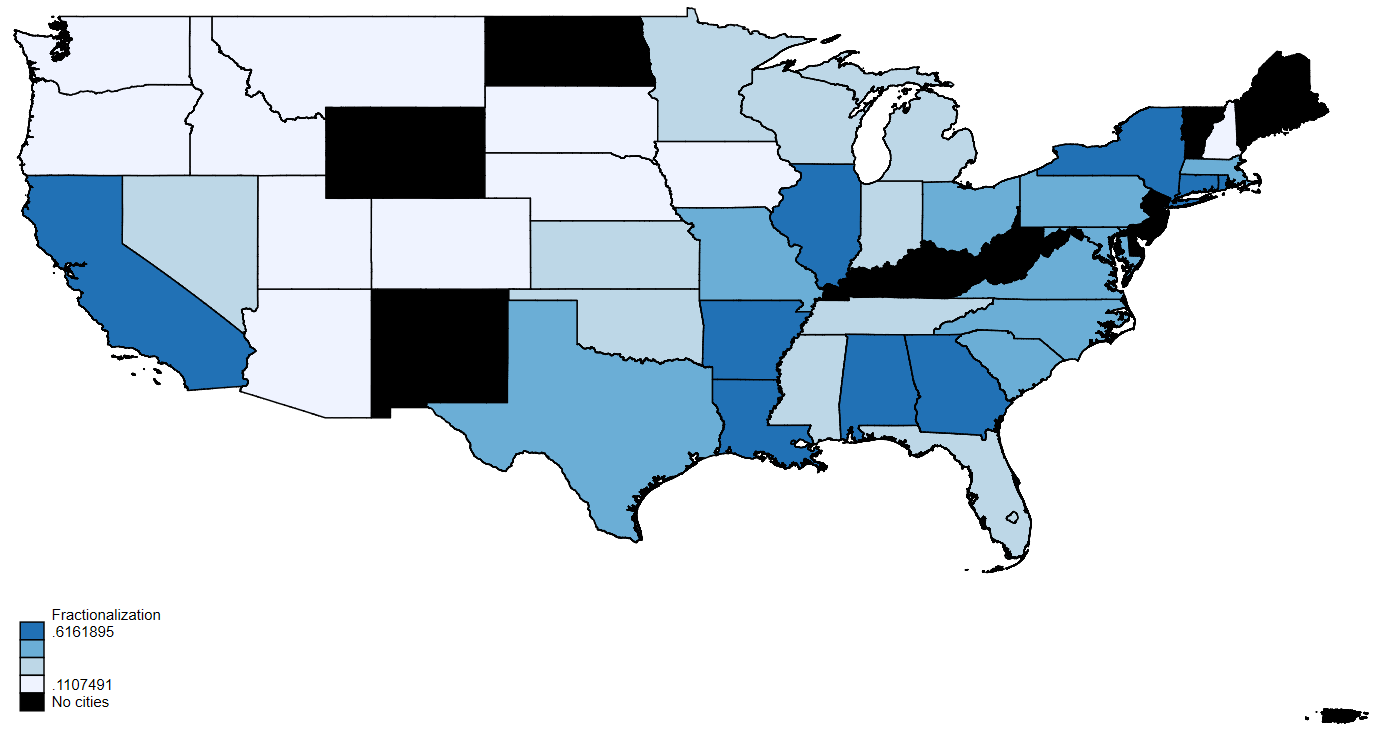
\includegraphics[scale = 0.3]{Thesis/Maps/state_frac.png}
    \caption{Fractionalization across state}
    \label{fig:frac_map}
\end{figure}

\begin{figure}[h!]
    \centering
    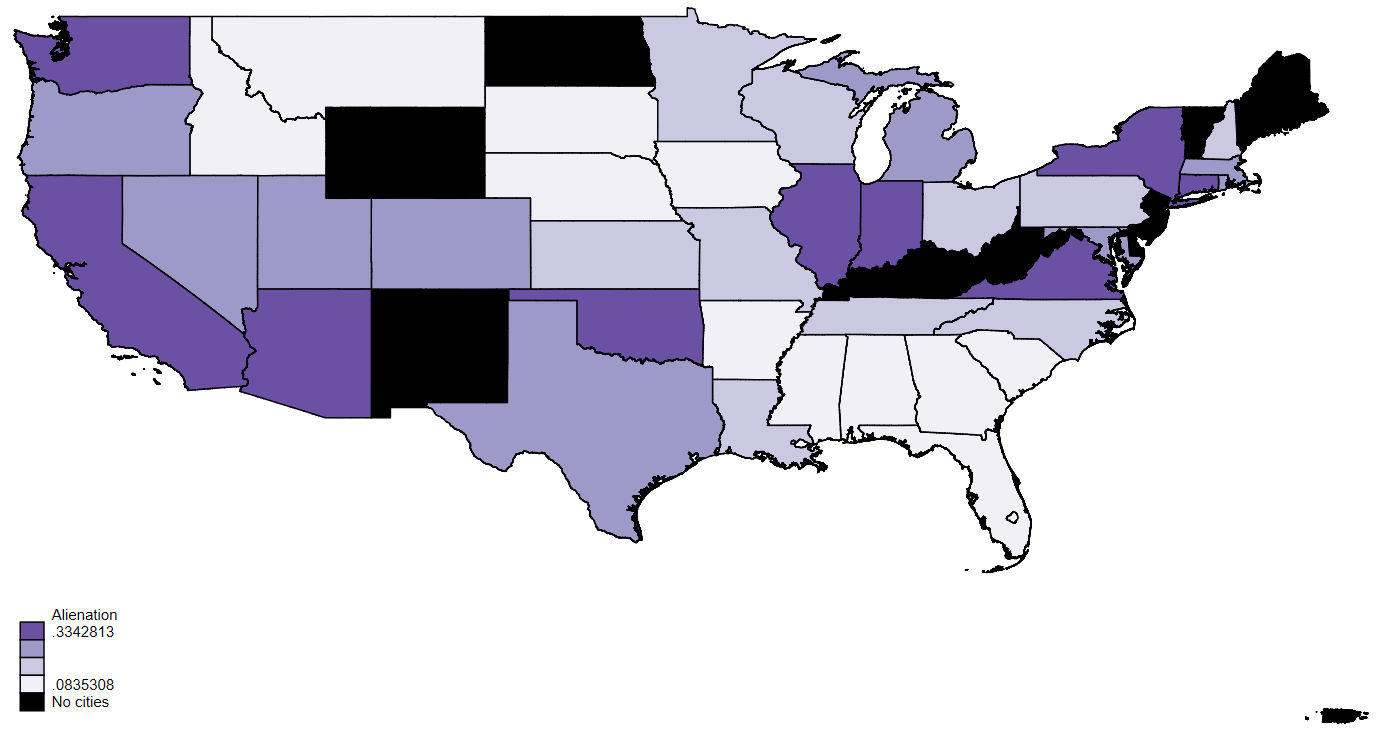
\includegraphics[scale = 0.3]{Thesis/Maps/state_index.png}
    \caption{Alienation across state}
    \label{fig:frac_map}
\end{figure}

\begin{figure}[h!]
    \centering
    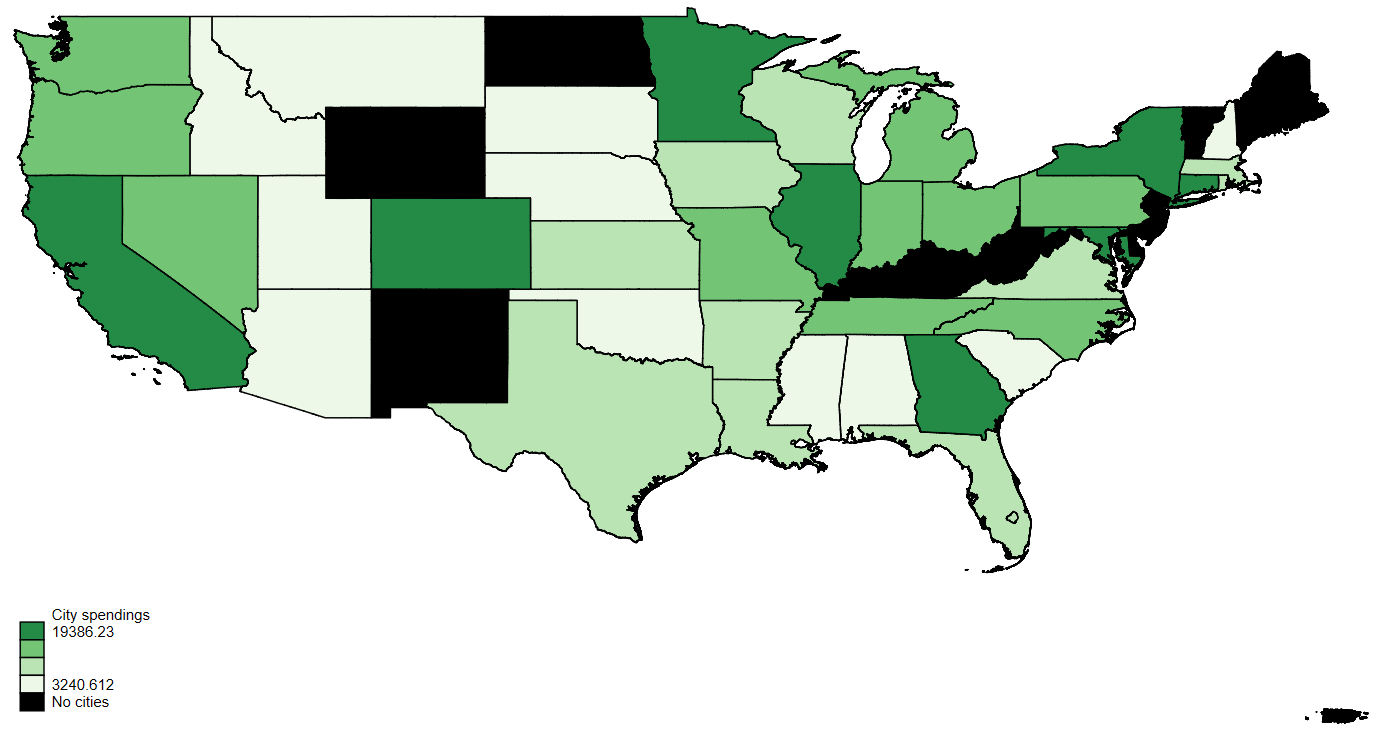
\includegraphics[scale = 0.3]{Thesis/Maps/state_spend.png}
    \caption{Spending across state}
    \label{fig:frac_map}
\end{figure}

\begin{figure}[h!]
    \centering
    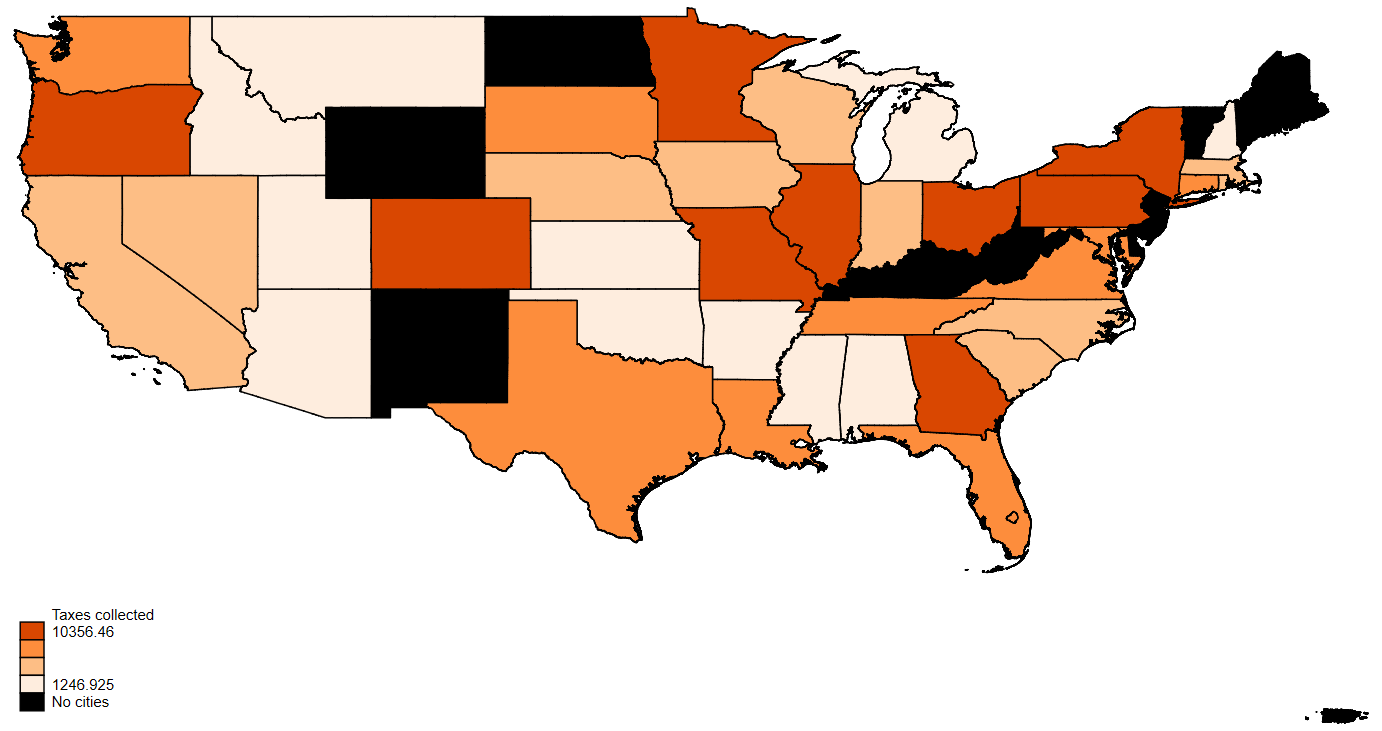
\includegraphics[scale = 0.3]{Thesis/Maps/state_taxes.png}
    \caption{Taxes across state}
    \label{fig:frac_map}
\end{figure}

\newpage
\section{Dose-response functions}

\begin{figure}[h!]
    \centering
    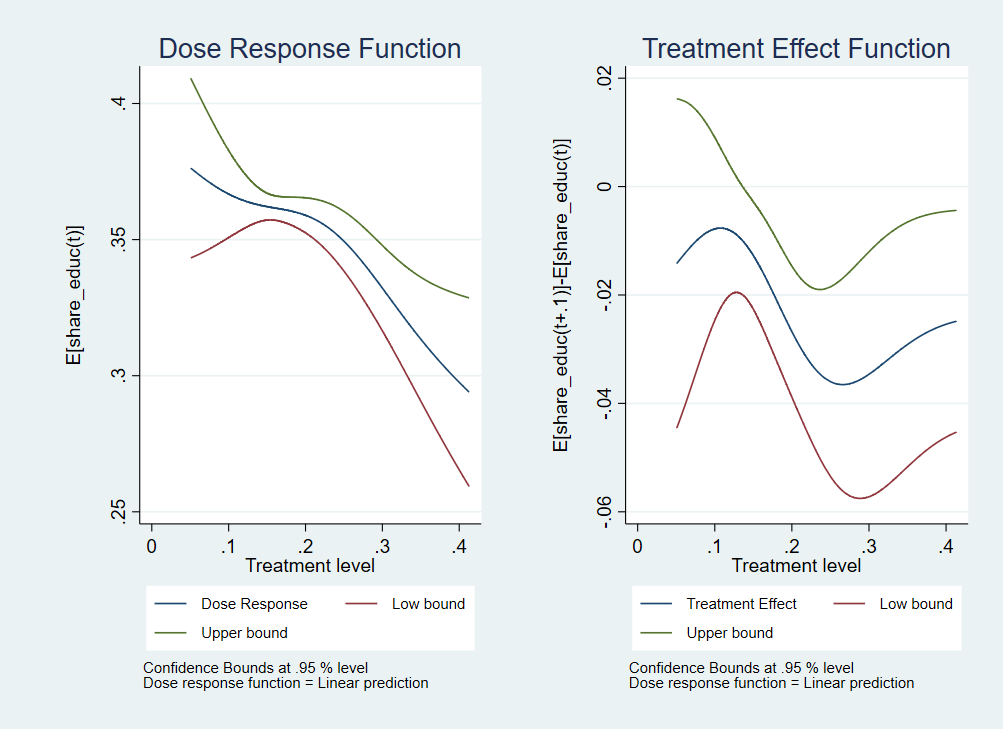
\includegraphics[scale = 0.4]{Thesis/Figures/graph_educ.png}
    \caption{Dose-response function (left) and its derivative (right) for secondary education spending}
    \label{fig:graph_educ}
\end{figure}

\begin{figure}[h!]
    \centering
    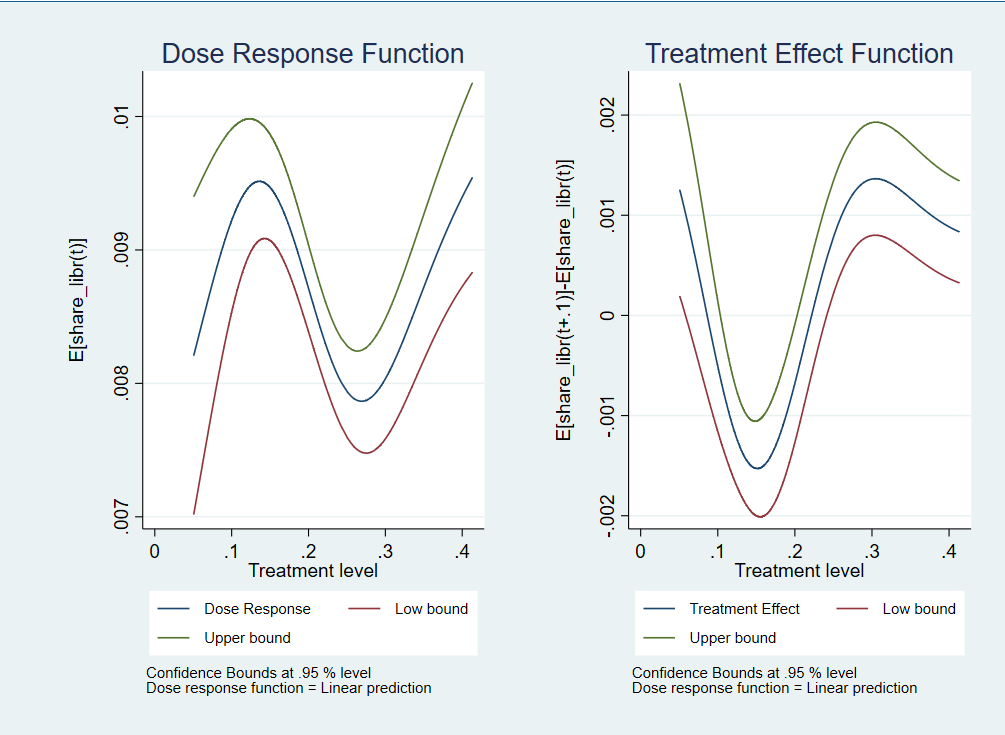
\includegraphics[scale = 0.4]{Thesis/Figures/graph_libr.png}
    \caption{Dose-response function (left) and its derivative (right) for library spending}
    \label{fig:graph_educ}
\end{figure}

\begin{figure}[h!]
    \centering
    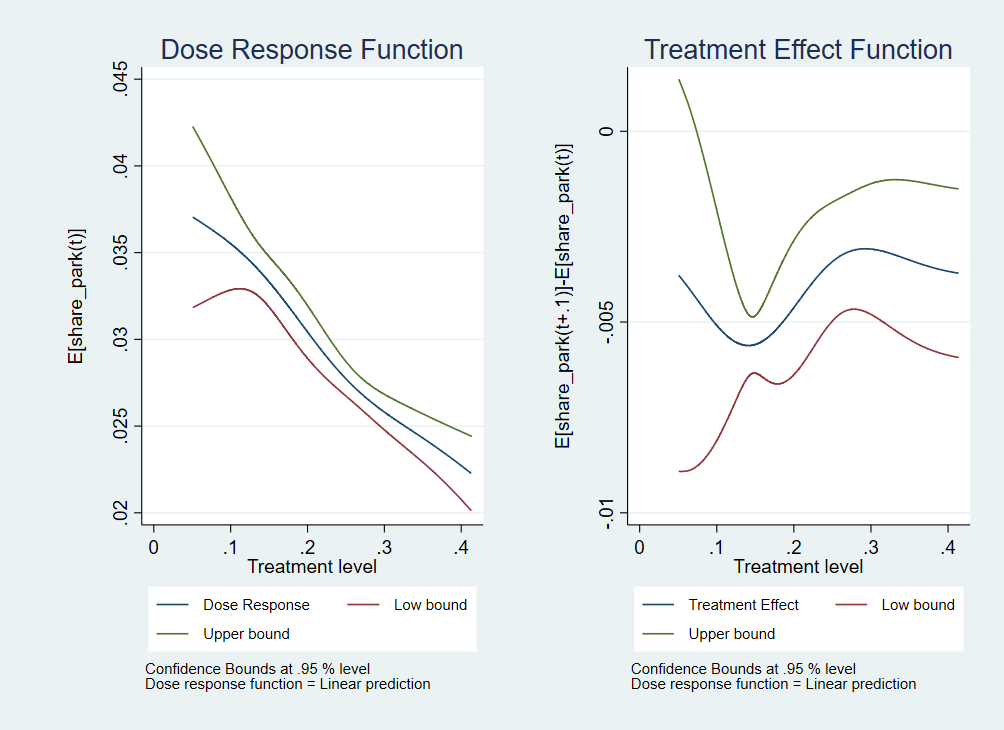
\includegraphics[scale = 0.4]{Thesis/Figures/graph_parks.png}
    \caption{Dose-response function (left) and its derivative (right) for parks and recreational spending}
    \label{fig:graph_educ}
\end{figure}

\begin{figure}[h!]
    \centering
    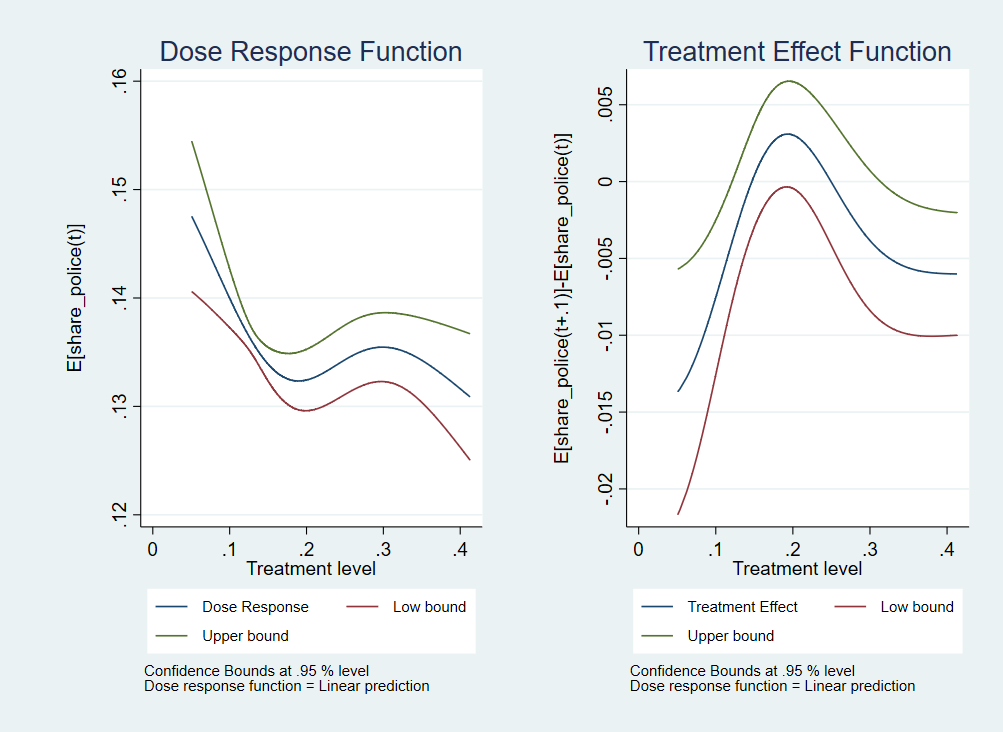
\includegraphics[scale = 0.4]{Thesis/Figures/graph_police.png}
    \caption{Dose-response function (left) and its derivative (right) for police spending}
    \label{fig:graph_educ}
\end{figure}

\begin{figure}[h!]
    \centering
    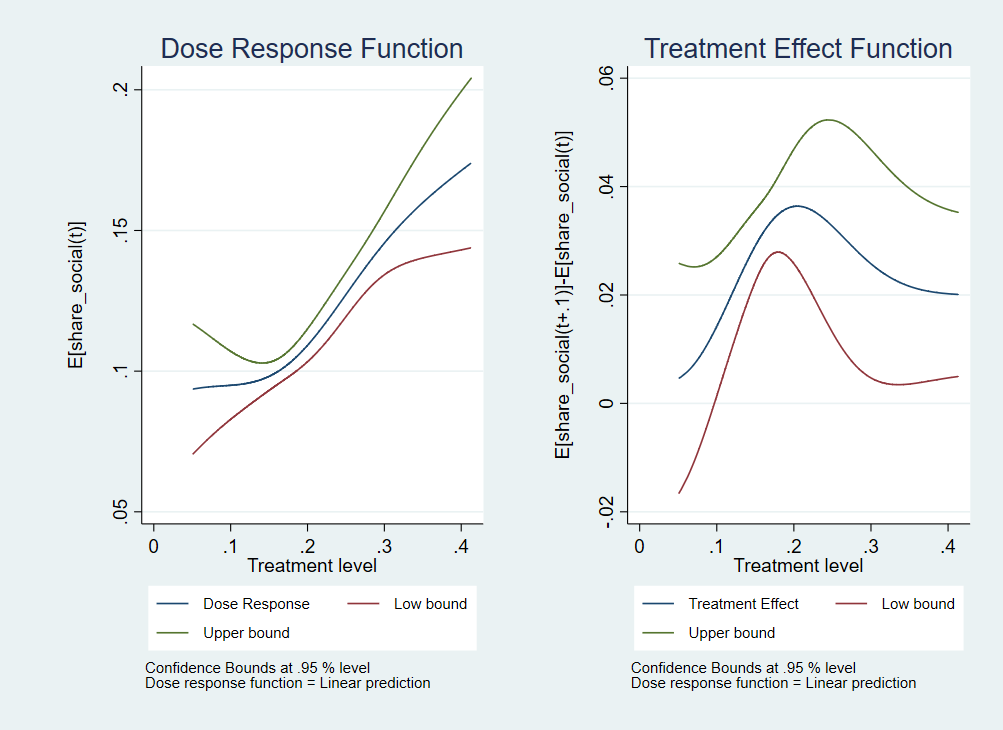
\includegraphics[scale = 0.4]{Thesis/Figures/graph_social.png}
    \caption{Dose-response function (left) and its derivative (right) for social spending}
    \label{fig:graph_educ}
\end{figure}

\begin{figure}[h!]
    \centering
    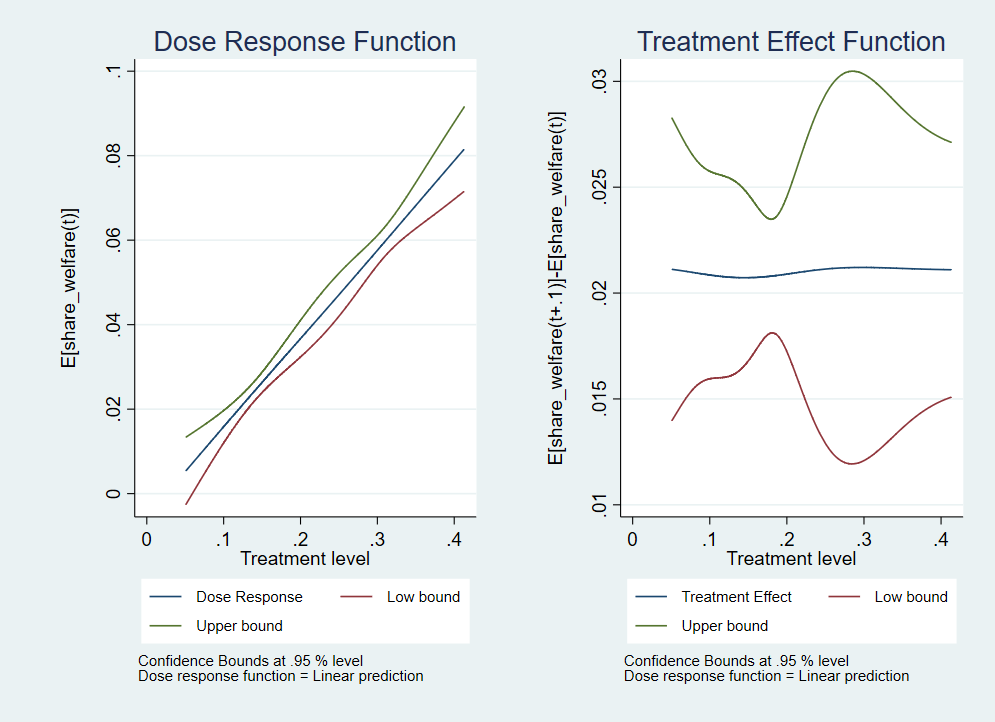
\includegraphics[scale = 0.4]{Thesis/Figures/graph_welfare.png}
    \caption{Dose-response function (left) and its derivative (right) for welfare spending}
    \label{fig:graph_educ}
\end{figure}


\end{document} 